%%
%% Copyright 2007-2024 Elsevier Ltd
%%
%% Working paper: Agri-CNX-Edge for Smart Agricultural Technology.
%% Derived from the pristine Elsarticle sample
%% (elsarticle-template-num.tex -- DO NOT EDIT the sample; edit THIS file).
%% Formatting follows the sample's rules only.
%%
%% NOTE FOR Scientific Reports (Springer Nature, CC BY, fully open access, Q1):
%% First submission may be single PDF/LaTeX; revised manuscript must use the
%% Springer Nature LaTeX template (sn-jnl) single-column, Nature refs [1],
%% Intro/Results/Discussion/Methods order. This file keeps elsarticle only
%% for review compilation; content below already follows Sci Rep limits:
%% title <=20 words, abstract <=200 words unstructured, keywords <=6,
%% displays consolidated to 8 with rest to Supplementary.
%% COVER LETTER DRAFT (paste into submission system; do not compile):
%% - Corresponding: Ankur Goyal, Dept CSE, SIT, SIU Pune India, ankur.goyal@sitpune.edu.in.
%% - Why Sci Rep: original engineering + biological-sciences system; technically sound
%%   unified offline apple monitoring with measured edge profile; fits Precision
%%   agriculture and smart farming Collection [COLLECTION-NAME-TO-BE-INSERTED].
%% - Suggested reviewers: [3 NAMES-EMAILS-AFFILIATIONS-TO-BE-INSERTED].
%% - Excluded reviewers: [UP-TO-3 NAMES/LABS-TO-BE-INSERTED, optional].
%% - Prior discussion with Board Member: [NONE/DETAILS-TO-BE-INSERTED].
%% - Prior submission: desk-rejected at Plant Methods for language only, no peer review;
%%   fully rewritten, new venue, all data/code statements included.
%% PRE-SUBMIT CHECKLIST (fill before submission; search TO-BE-INSERTED):
%% [ ] GitHub private URL + commit hash + env versions; reviewer ZIP as Supplementary.
%% [ ] Zenodo DOI placeholder; dataset links/licenses/access dates; pHash library version.
%% [ ] SAM + X-AnyLabeling versions + verifier initials/protocol; PDDD full name/source.
%% [ ] Grant number if applicable; Collection name; 3 suggested + excluded reviewers.
%% [ ] Beyond main.tex (not done here): 3-seed reruns with SD/CIs, complete static run,
%%     best-checkpoint re-eval, single-task baselines, INT8 estimate, Nature ref conversion,
%%     move excess displays to Supplementary, professional language edit as final step.
\documentclass[preprint,12pt,numafflabel]{elsarticle}
%% Forced sample-style title block: the automatic affiliation marker is
%% silenced because the shared address carries manual 1,2,3,4,5 marks.
\AtBeginDocument{\def\theaffn{}}

%% Use the option review to obtain double line spacing
%% \documentclass[authoryear,preprint,review,12pt]{elsarticle}

%% Use the options 1p,twocolumn; 3p; 3p,twocolumn; 5p; or 5p,twocolumn
%% for a journal layout:
%% \documentclass[final,1p,times]{elsarticle}
%% \documentclass[final,1p,times,twocolumn]{elsarticle}
%% \documentclass[final,3p,times]{elsarticle}
%% \documentclass[final,3p,times,twocolumn]{elsarticle}
%% \documentclass[final,5p,times]{elsarticle}
%% \documentclass[final,5p,times,twocolumn]{elsarticle}

%% For including figures, graphicx.sty has been loaded in
%% elsarticle.cls. If you prefer to use the old commands
%% please give \usepackage{epsfig}

%% The amssymb package provides various useful mathematical symbols
\usepackage{amssymb}
%% The amsmath package provides various useful equation environments.
\usepackage{amsmath}
%% The amsthm package provides extended theorem environments
%% \usepackage{amsthm}

%% Tables with professional rules (appendix-free, review-safe)
\usepackage{booktabs}
%% Wrapping columns for narrow review text width
\usepackage{tabularx}
\usepackage{array}
\usepackage{xltabular}
\usepackage{ragged2e}
\usepackage{url}
%% Tight, aligned lists
\usepackage{enumitem}
%% Keep floats inside their sections (no drift past References)
\usepackage{placeins}
%% Vector schematics drawn in-paper (fonts match body text)
\usepackage{tikz}
\usetikzlibrary{arrows.meta,positioning,shapes.geometric,calc,backgrounds}

%% Line numbers disabled per author request (enable for peer review if needed).
%% \usepackage{lineno}

\journal{}

\begin{document}

\begin{frontmatter}

%% Title, authors and addresses

%% use the tnoteref command within \title for footnotes;
%% use the tnotetext command for theassociated footnote;
%% use the fnref command within \author or \affiliation for footnotes;
%% use the fntext command for theassociated footnote;
%% use the corref command within \author for corresponding author footnotes;
%% use the cortext command for theassociated footnote;
%% use the ead command for the email address,
%% and the form \ead[url] for the home page:
%% \title{Title\tnoteref{label1}}
%% \tnotetext[label1]{}
%% \author{Name\corref{cor1}\fnref{label2}}
%% \ead{email address}
%% \ead[url]{home page}
%% \fntext[label2]{}
%% \cortext[cor1]{}
%% \affiliation{organization={},
%%             addressline={},
%%             city={},
%%             postcode={},
%%             state={},
%%             country={}}
%% \fntext[label3]{}

\title{One shared DINOv3-ConvNeXt model unifies apple disease, pest, grading and counting offline}

\author{Aarya Balwadkar\textsuperscript{1}, Afifa Bintul Hasan\textsuperscript{1}, Eccha Bansal\textsuperscript{1}, Aparna Nair\textsuperscript{1} and Ankur Goyal\textsuperscript{1,*}}

%% Author affiliation
\affiliation[]{organization={Department of Computer Science and Engineering,
    Symbiosis Institute of Technology, Symbiosis International (Deemed University)},
            city={Pune},
            state={Maharashtra},
            country={India\\[4pt]*Corresponding author. E-mail: ankur.goyal@sitpune.edu.in\\[4pt]Contributing authors: aarya.balwadkar2005@gmail.com, hasanafifabintul@gmail.com, bansalagrawaleccha@gmail.com, aparna@gmail.com}}

%% Abstract
\begin{abstract}
Field diagnosis of apple problems usually needs separate models for leaf disease, insect pests, fruit grading and fruit counting, repeating the same image analysis on hardware that cannot afford it. We present a single shared vision model that performs all four tasks offline on a low-cost phone. The model uses a DINOv3-pretrained ConvNeXt-Tiny backbone with low-rank adaptation, task-specific heads and adaptive weighting of task losses. On held-out test images it correctly classifies 100\% of leaf cases (623 images) and 99.6\% of pest cases (225 images), grades fruit disease at 95.7\% on ground-truth fruit regions, and counts apples with mean absolute error 3.5 apples per image and correlation 0.85 on 400 orchard images. Adaptive weighting is essential: equal weighting reduces fruit accuracy to 70.3\%. Teacher-student distillation provides no gain when teachers are saturated. The 120.7 megabyte model runs fully offline in about 5.6 seconds per image. This shows unified offline apple monitoring is feasible, with counting in dense clusters as the remaining limit.
\end{abstract}

%%Graphical abstract
% \begin{graphicalabstract}
% \includegraphics[width=\textwidth]{figures/grabs.jpg}
% \end{graphicalabstract}

%%Research highlights
% \begin{highlights}
% \item Unified 4-task apple AI runs fully offline on a budget phone
% \item Adaptive weighting is essential; static weights collapse fruit to 70\%
% \item Distillation does not help under saturated teachers: No-KD wins all
% \item Measured edge profile: 120.7\,MB, ${\sim}5.6$\,s, identical providers
% \end{highlights}

%% Keywords
\begin{keyword}
Precision agriculture \sep Multi-task learning \sep Edge computing \sep Plant disease detection \sep Fruit counting \sep Knowledge distillation
\end{keyword}

\end{frontmatter}

%% \linenumbers (disabled per author request)

%% main text
%%

\FloatBarrier
\section{Introduction}
\label{sec:introduction}

Agriculture plays a critical role in food security, economic
development, and sustainable resource management. Crop diseases, pest
infestations, and inaccurate assessment of fruit production
significantly affect crop quality and productivity, and computer
vision offers a path to automate disease recognition, pest
identification, fruit classification, fruit localization, and fruit
counting.

Deep learning has become an important approach for agricultural image
analysis because it learns discriminative visual representations
directly from images. Convolutional networks, transfer learning,
object detection, and self-supervised representation learning have
demonstrated strong performance across agricultural applications.

However, most deployed systems are single-task: a
disease-classification model, a pest-detection model, and a
fruit-counting model each extract their own features independently.
On resource-constrained hardware this means repeated computation,
higher memory, and a deployment story that does not scale to the
field. Multi-task learning promises an alternative -- several related
tasks sharing one visual representation -- but agricultural tasks
disagree in output structure and loss character: leaf and pest
recognition are image-level classification while fruit counting is
inherently spatial. Two further assumptions in the literature deserve
testing rather than trust: that teacher distillation necessarily helps
the student, and that on-device deployment follows from a small
checkpoint. This work tests both claims with measurements.

Agri-CNX-Edge addresses the problem with a shared DINOv3-pretrained ConvNeXt-Tiny
visual backbone with low-rank adaptation (LoRA), hierarchical feature
routing, a feature pyramid network-lite neck (FPN-Lite), lightweight task-specific heads, a decoupled
anchor-free you only look once (YOLO) detection head with region of interest Align (ROI-Align)-based per-apple
classification, heterogeneous knowledge distillation, and adaptive
weighting of task losses based on homoscedastic uncertainty -- all evaluated on device on a budget
smartphone.

The principal contributions of this work are:

\begin{itemize}[leftmargin=*,itemsep=2pt,parsep=2pt]

\item A unified multi-task architecture for leaf disease classification,
pest recognition, fruit classification and fruit localization with
counting that runs fully offline on device.

\item Hierarchical feature routing in which fine-grained features serve
leaf classification, mid-scale features serve pest recognition and
fused multi-scale features serve apple detection, with per-apple fruit
classification from ROI-Align crops as defined in Section~\ref{sec:methodology}.

\item A heterogeneous distillation strategy that combines categorical
distillation for classification with box-level distillation for
detection, reported with the measured finding that it does not improve
the student under saturated teachers.

\item A teacher pipeline with three classification seeds and eight
augmentation views per seed, complemented by a YOLO26s detection
teacher for bounding-box supervision.

\item Adaptive uncertainty weighting for heterogeneous objectives,
validated as essential because static weighting collapses fruit test
accuracy to 70.26\%.

\item A structured ablation of distillation, weighting, adaptation and
warm-up with measured deployment evidence on a Samsung A17 5G with
identical numerics across providers.

\end{itemize}

The remainder of the paper follows this contribution order as a single
narrative: Section~\ref{sec:related} and Table~\ref{tab:related} show
why prior work leaves the gap open, Section~\ref{sec:gap} formalizes
the gap, Section~\ref{sec:methodology} with Figs.~\ref{fig:arch}--\ref{fig:loss}
and Eqs.~\ref{eq:seeds}--\ref{eq:total} builds the Agri-CNX-Edge answer
centered on DINOv3, Sections~\ref{sec:dataset}--\ref{sec:experimental} fix data
and measurement, Section~\ref{sec:results} with
Tables~\ref{tab:final_results}--\ref{tab:edge} tests each claim, and
Sections~\ref{sec:discussion}--\ref{sec:limitations} synthesize what
survived measurement.

\FloatBarrier
\section{Related Work}
\label{sec:related}

This section reviews only work directly relevant to a unified
multi-task model that runs offline on a phone. It proceeds from
agricultural multi-task systems to offline mobile systems and finally
to the representations and training mechanisms that make unification
possible. Table~\ref{tab:related} summarises the comparison and is
discussed at the end of the section.

\subsection{Multi-Task Learning in Agriculture}

Single-task apple models remain common, such as real-time apple leaf
systems~\cite{khan2022} and orchard detection and counting
pipelines~\cite{gao2022}. The literature after 2020 moves beyond them
toward joint models. Luan et al.\ proposed ALMDR, a multi-task apple
leaf model that jointly performs multi-label classification,
detection, segmentation and severity estimation with a group feature
pyramid, reporting 93.74\% F1-score, 51.32\% detection mean average precision (mAP) and severity
coefficient of determination ($R^2$) 0.9757 at 6.25 frames per second (fps)~\cite{luan2025}. Kang et al.\
proposed a lightweight tomato model that jointly performs leaf disease
detection and fruit counting~\cite{kang2024}, the closest precedent to
combining classification with counting. PMJDM jointly performs plant
species classification and disease detection from a shared ConvNeXt
backbone with dynamic weight adjustment, reporting 71.84\% precision
and 61.83\% mAP at IoU 0.50 (mAP50) at 113 fps with 49.1M
parameters~\cite{pmjdm2025}. PlantSDS-Net jointly performs species,
disease and severity classification in one model with task attention,
reporting 99.89\%, 99.58\% and 92.18\% on the three
tasks~\cite{plantsds2026}. Beyond classification, CMTL unifies cotton
boll detection, pest damage segmentation and growth stage
classification in one transformer with cross-level encoding, reporting
0.913 mAP, 0.832 Intersection over Union (IoU) and 0.936 accuracy with Jetson Xavier NX edge
trials~\cite{cmtl2025}. For joint disease and pest recognition, a
DenseNet-121 and ResNet-50 fusion reports 99.13\% disease and 98.67\%
pest accuracy~\cite{sood2025}, while DAM-Net uses a discriminative
attention network with ResNet-50 and adaptive weighted loss to reach
99.7\% on the D0 pest dataset and 74.1\% on the IP102 large-scale insect pest dataset with 102 categories~\cite{damnet2024}. Pest-YOLO jointly
addresses dense tiny pest detection and counting with focal loss and a
confluence strategy, reporting 69.59\% mAP and counting root mean square error (RMSE)
0.44~\cite{wen2022}. Together these studies prove that sharing
features across agricultural tasks is feasible, but none combines leaf
disease, pest, fruit grading and spatial counting in one DINOv3 edge
model with tested task weighting.

\subsection{Mobile and Offline Edge AI in Agriculture}

Field deployment requires offline inference on low-end phones, a
constraint addressed explicitly only after 2020. PlanteSaine integrates
EfficientNetB3 with an artificial neural network classifier into an
Android app with TensorFlow Lite and offline operation for maize,
tomato and onion farmers in Burkina Faso~\cite{plante2024}. At
model level, an ultra-lightweight network reports competitive plant
disease and pest accuracy with fewer than 150,000
parameters~\cite{wang2023ulen}, and a MobileNetV3-small edge model
reports 99.50\% accuracy after quantization to 0.93M parameters in
Open Neural Network Exchange (ONNX) format at 100 frames per second on
central processing unit (CPU)~\cite{schuler2022edge}. These systems establish that offline
mobile diagnosis is achievable, but they remain single-task
classifiers without unified counting, without heterogeneous
distillation and without measured multi-task ablation.

\subsection{Foundation Representations, Distillation and Task Balancing}

DINOv2-FCS builds fruit leaf classification and severity prediction on
a DINOv2-B backbone with class-patch fusion and explicit multi-scale
fusion, reporting 99.67\% classification accuracy, 90.29\% mean Intersection over Union (mIoU) and
95.68\% severity accuracy, with mobile deployment listed as future
work~\cite{bai2024dinov2}. EConv-ViT fuses ConvNeXt and Vision
Transformer (ViT) with channel attention for apple leaf disease, reporting
99.2\% in lab and 79.3\% in natural
conditions~\cite{huang2025econv}. DINOv3 scales self-supervision to 7B
parameters and 1.7B images and distils to ConvNeXt Tiny, Small, Base
and Large variants for resource-constrained
deployment~\cite{simeoni2025}. This work uses the Tiny variant as the
shared representation. For training, distillation is also shown in lightweight plant
models~\cite{huang2023}, and task balancing follows homoscedastic
uncertainty weighting~\cite{kendall2018} as the lightest alternative
to gradient normalization~\cite{chen2018} and conflict-averse
updates~\cite{liu2021cagrad}. On-device benchmarking follows
MLPerf Mobile~\cite{reddi2022} and
MDLBench practice~\cite{liumd2022} with a uniform app, model, images
and code per device. This paper follows the same discipline while
reporting the reduced sample tail honestly.

\subsection{Orchard-Scale Detection and Counting}

Counting is the spatial half of the gap, and orchard literature treats it
as a detection problem first and an arithmetic problem second. Jin et al.\ enhance you only look once v8 nano (YOLOv8n)
with re-parameterized blocks, a generalized feature pyramid and a new
Intersection over Union (IoU) loss for robotic harvesting, reaching 81.68\% mAP50 with counting
accuracy 69.39\% and millimetre-level localization under varied lighting
and occlusion~\cite{jin2025}. This study proves that modern YOLO
detectors survive orchard clutter, yet it stops at detection plus
counting without leaf, pest or grading tasks. For temporal context, Hani et
al.\ comparatively benchmark detection against tracking-based yield mapping
methods in apple orchards~\cite{hani2020}. This work establishes that
frame-to-frame association matters as much as per-frame precision, a lesson
this work inherits through decoded-box counting even though it counts from
single images rather than video. Taken together, the
detection literature offers mature spatial machinery with measured mean absolute error (MAE) and
RMSE discipline that this work adopts, but no study routes detection
features onward into per-apple grading inside one shared backbone.

\subsection{Datasets, Single-Task Foundations and Field Realism}

No multi-task claim is credible without naming the data it stands on. The
PlantVillage repository of over 54,000 controlled leaf images across 38
classes underpins modern classification work~\cite{mohanty2016}. Early reviews map the
territory: Ferentinos surveys deep models for disease detection and
diagnosis~\cite{ferentinos2018}, Dhaka et al.\ survey convolutional
networks for leaf disease prediction~\cite{dhaka2021}, and Liu and Wang
review deep learning for joint plant disease and pest
detection~\cite{liu2021}. Recent syntheses raise the bar further: Shoaib et
al.\ review deep learning for plant disease and pest detection and report
classification accuracies above 95\% with detection precision above 90\% in
controlled settings~\cite{shoaib2025}, while Banerjee et al.\ taxonomize
hyperspectral, visualisation, modified deep and transformer methods and
show hierarchical vision transformers above 99.3\% against MobileNetV3
baselines~\cite{banerjee2025}. For pests at scale, the IP102 dataset of
102 pest categories anchors realistic infestation
modelling~\cite{wu2019ip102}. The persistent warning across all these
sources is field realism: Picon et al.\ show mobile-captured in-the-wild
crop images degrade lab-trained classifiers and propose device-aware
training~\cite{picon2018}, Janarthan et al.\ build an in-field mobile
solution for palm pathology~\cite{janarthan2022}, and Picon et al.\ extend
to crop-conditional networks over cell-phone images taken under real field
conditions~\cite{picon2019}. This work therefore treats lab accuracy as a
ceiling signal and field robustness as the binding constraint, which is why
evaluation separates controlled classification from cluttered counting.

\subsection{Backbones, Compression and Balancing Protocols}

The backbone lineage behind Agri-CNX-Edge is itself a literature. Residual
learning made very deep networks trainable~\cite{he2016}, ConvNeXt
modernized pure ConvNets with transformer-inspired design while keeping
convolutional efficiency~\cite{liu2022}, and shifted-window transformers
added hierarchical attention with efficient local-global
trade-offs~\cite{swin2021}. Self-supervision then removed the label
bottleneck: vision transformers showed patches plus attention suffice at
scale~\cite{dosovitskiy2020}, DINO revealed emergent object structure in
self-supervised transformers~\cite{caron2021}, and DINOv2 delivered robust
frozen features without supervision~\cite{oquab2023}, culminating in the
DINOv3 family used here. Efficiency has a parallel lineage: EfficientNet
compounds scaling for accuracy per parameter~\cite{tan2019} and MobileNetV3
optimizes for phone CPUs through hardware-aware
search~\cite{howard2019}. Detection contributes its own primitives: the
unified real-time YOLO formulation~\cite{redmon2016} with its community
YOLOv5 release~\cite{jocher2020} and feature pyramids for multi-scale
fusion~\cite{lin2017}, all of which echo in the decoupled anchor-free head
and FPN-Lite neck of this work. Adaptation and compression close the loop
to the edge: low-rank adaptation inserts tiny trainable matrices into
frozen weights~\cite{hu2021}, deep compression prunes and shares
parameters for deployment~\cite{han2016}, and integer-arithmetic-only
quantization enables on-device inference~\cite{jacob2018}. For balancing, the survey by Vandenhende et
al.\ systematises multi-task dense prediction trade-offs~\cite{vandenhende2022},
alongside multi-objective optimization~\cite{sener2018} and gradient
surgery for conflicting gradients~\cite{yu2020} as heavier alternatives to
the homoscedastic weighter adopted here. The conjunction this work tests --
one DINOv3 backbone, heterogeneous categorical plus spatial distillation,
adaptive weighting and measured phone deployment -- appears in none of
these sources combined.

Table~\ref{tab:related} consolidates studies directly relevant to
multi-task or offline mobile agriculture, now spanning more than fifty
cited sources across the section. Table~\ref{tab:related} shows
the upper block compares twelve agricultural multi-task systems, the
second block compares two offline mobile systems, the third block
compares two orchard detection and counting systems, and the lower block
places the DINO representation lineage used here. Across the upper block,
reported strengths are real, yet narrow: Wen et al.\ report 69.59\% mAP
with RMSE 0.44 for dense pest detection and counting, DAM-Net reaches
99.7\% on the D0 pest dataset with adaptive loss, Luan et al.\ report F1-score 93.74\% at 6.25
fps for apple leaf tasks, and EConv-ViT fuses ConvNeXt with Transformer
for apple leaves, while Kang et al.\ provide the closest precedent by
joining leaf disease with fruit counting, though only for tomato without
pest, grading or DINOv3. The second block shows that offline operation is
solved in isolation: PlanteSaine and the
MobileNetV3-small edge model run on constrained hardware, with the quantized
MobileNetV3-small at 0.93M parameters and 100 fps, yet each
remains without unified counting, heterogeneous distillation or
multi-task ablation. The third block contributes the spatial machinery
this work borrows: Jin et
al.\ harden YOLOv8n for harvesting at 81.68\% mAP50 and Hani et al.\ benchmark yield-mapping methods
-- both detection plus counting, neither
routing detection features into grading. The lower block traces the
representation shift from DINOv2-B fusion at 99.67\% accuracy without
counting or mobile proof to DINOv3 pretraining distilled to ConvNeXt
Tiny, which this work adopts as the shared backbone. Read across the
Result and Limitation columns, no listed system combines four apple
tasks in one DINOv3 backbone with heterogeneous distillation, tested
adaptive weighting and measured offline phone deployment. That
conjunction is the gap formalized in Section~\ref{sec:gap}.

\footnotesize
\setlength{\tabcolsep}{3pt}
\renewcommand{\arraystretch}{1.18}
\setlength{\emergencystretch}{6pt}
\begin{xltabular}{\textwidth}{@{}>{\RaggedRight\arraybackslash\hspace{0pt}}p{2.1cm} c >{\RaggedRight\arraybackslash\hspace{0pt}}X >{\RaggedRight\arraybackslash\hspace{0pt}}X >{\RaggedRight\arraybackslash\hspace{0pt}}X >{\RaggedRight\arraybackslash\hspace{0pt}}X@{}}
\caption{Related work directly relevant to multi-task agriculture, offline mobile deployment and orchard counting. Upper block: agricultural multi-task systems. Second block: offline mobile systems. Third block: orchard detection and counting systems. Lower block: DINO lineage used in this work.}
\label{tab:related}\\
\toprule
\textbf{Study} & \textbf{Year} & \textbf{Tasks unified} & \textbf{Backbone and edge form} & \textbf{Reported result} & \textbf{Limitations} \\
\endfirsthead
\caption*{Table~\ref{tab:related} (continued)}\\
\toprule
\textbf{Study} & \textbf{Year} & \textbf{Tasks unified} & \textbf{Backbone and edge form} & \textbf{Reported result} & \textbf{Limitation vs.\ this work} \\
\midrule
\endhead
\midrule
\multicolumn{6}{r@{}}{\footnotesize\textit{Continued on next page}} \\
\endfoot
\bottomrule
\endlastfoot
\midrule
\multicolumn{6}{@{}l}{\textit{Agricultural multi-task systems}} \\
\midrule
Wen et al.~\cite{wen2022} & 2022 & Pest detection + counting & YOLOv4 + focal + confluence & 69.59\% mAP; RMSE 0.44 & Pest only; no disease/fruit; no phone measure \\
Khan et al.~\cite{khan2022} & 2022 & Apple leaf disease & CNN real-time detector & Real-time leaf & Single task; no pest/fruit/counting \\
Gao et al.~\cite{gao2022} & 2022 & Apple detection + counting & Detector + trunk tracking & Orchard pipeline & Counting only; no classification \\
DAM-Net~\cite{damnet2024} & 2024 & Pest recognition multi-task & Attention + ResNet-50, adapt.\ loss & 99.7\% D0; 74.1\% IP102 & Pest only; no detection; no edge \\
Kang et al.~\cite{kang2024} & 2024 & Leaf disease + fruit count & Lightweight joint model & Joint inspection & Tomato only; no pest/grading; no DINOv3 \\
Bai et al.~\cite{bai2024dinov2} & 2024 & Leaf classific.\ + severity & DINOv2-B + fusion & 99.67\%; 90.29\% mIoU & No counting; server GPU; mobile future \\
Sood et al.~\cite{sood2025} & 2025 & Disease + pest & DenseNet-121 + ResNet-50 & 99.13\%; 98.67\% & Two-task classifier; no counting; no edge \\
Luan et al.~\cite{luan2025} & 2025 & Apple disease + segment.\ & Group pyramid + heads & F1 93.74\%; 6.25 fps & Leaf only; no pest/counting \\
PMJDM~\cite{pmjdm2025} & 2025 & Species + disease detect.\ & ConvNeXt + dynamic weights & 61.83\% mAP50; 113 fps & No grading/counting; no phone \\
CMTL~\cite{cmtl2025} & 2025 & Boll + pest + stage & Transformer + Jetson Xavier NX & 0.913 mAP; 0.832 IoU & Cotton UAV; not apple phone \\
PlantSDS-Net~\cite{plantsds2026} & 2026 & Species + disease + severity & Res2Net + MobileNetV2 + attent.\ & 99.89\%; 99.58\%; 92.18\% & Classific.\ only; no counting/edge \\
EConv-ViT~\cite{huang2025econv} & 2025 & Apple leaf disease & ConvNeXt + Transformer + channel attent.\ & 99.2\% lab; 79.3\% field & Single task; lab-field gap; no edge \\
\midrule
\multicolumn{6}{@{}l}{\textit{Offline mobile systems}} \\
\midrule
PlanteSaine~\cite{plante2024} & 2024 & Maize/tomato/\ onion diagn.\ & EfficientNetB3 + ANN, TFLite & Offline app & Single-task; no counting/MTL \\
Schuler et al.~\cite{schuler2022edge} & 2023 & Plant disease edge & MobileNetV3-small ONNX quant.\ & 99.50\%; 0.93M; 100 fps & Single task; no MTL/counting \\
\midrule
\multicolumn{6}{@{}l}{\textit{Orchard detection and counting systems}} \\
\midrule
Jin et al.~\cite{jin2025} & 2025 & Apple detect.\ + count & Enhanced YOLOv8n + GIoU var.\ & 81.68\% mAP50; count 69.39\% & Harvesting only; no MTL \\
Hani et al.~\cite{hani2020} & 2020 & Fruit detect.\ + yield map & Compared detect.\ vs tracking & Benchmark of methods & Benchmark only; no system \\
\midrule
\multicolumn{6}{@{}l}{\textit{DINO representation lineage used here}} \\
\midrule
Simeoni et al.~\cite{simeoni2025} & 2026 & Foundation pretraining & DINOv3 7B to ConvNeXt Tiny & Frozen SOTA & Pretraining only; no apple system \\
This work & 2026 & Leaf + pest + fruit + count & DINOv3-ConvNeXt-Tiny LoRA, ONNX & Sec.~7--9, phone measured & Tested weighting; KD limit documented \\
\end{xltabular}

\FloatBarrier
\section{Research Gap}
\label{sec:gap}

Section~\ref{sec:related} and Table~\ref{tab:related} leave a precise
conjunction unresolved. Single-task studies leave repeated backbone
computation undeployed; multi-task work rarely spans classification
\emph{and} spatial counting with distillation for both; and edge claims
rarely come with phone measurements. The gap addressed here is
therefore the integration of heterogeneous tasks, hierarchical routing
(Eqs.~\ref{eq:routing-cls}--\ref{eq:routing-det}), categorical-plus-spatial
distillation (Eqs.~\ref{eq:kl}--\ref{eq:yield}), adaptive balancing
(Eqs.~\ref{eq:mtl}--\ref{eq:total}), and a measured on-device design --
with each component ablated rather than assumed. Section~\ref{sec:methodology}
implements this integration step-by-step, so every gap item has a
corresponding methodological answer.

\FloatBarrier
\section{Methodology}
\label{sec:methodology}

This section answers the gap item-by-item in the order it was posed:
overview mapping to Fig.~\ref{fig:arch}, teachers supplying
Eqs.~\ref{eq:seeds}--\ref{eq:tta-avg}, distillation formalized in
Eqs.~\ref{eq:kl}--\ref{eq:yield}, backbone and routing in
Eqs.~\ref{eq:features}--\ref{eq:routing-det}, and heads with
optimization in Eqs.~\ref{eq:heads}--\ref{eq:total}. Nothing that
follows is incidental; each subsection exists because the previous
figure or equation requires it.

\subsection{System Overview}

Agri-CNX-Edge consists of five major components:

\begin{enumerate}[leftmargin=*,itemsep=2pt,parsep=2pt]

\item Dataset curation and preprocessing with cleaning, stratified
70/15/15 splits and task-specific augmentation.

\item Specialized teacher models with ConvNeXt-Small classification teachers
fine-tuned from a 120-class Plant Disease Dataset checkpoint (PDDD) [FULL-NAME-AND-SOURCE-TO-BE-INSERTED] and a YOLO26s
apple-detection teacher.

\item Shared DINOv3-ConvNeXt-Tiny student backbone with low-rank adaptation (LoRA) adapters.

\item Feature pyramid network-lite neck (FPN-Lite) and hierarchical feature routing.

\item Task-specific classification heads, a decoupled you only look once (YOLO) detection
head, and region of interest Align (ROI-Align)-based per-apple fruit classification.

\end{enumerate}

\begin{figure}[htbp]
\centering
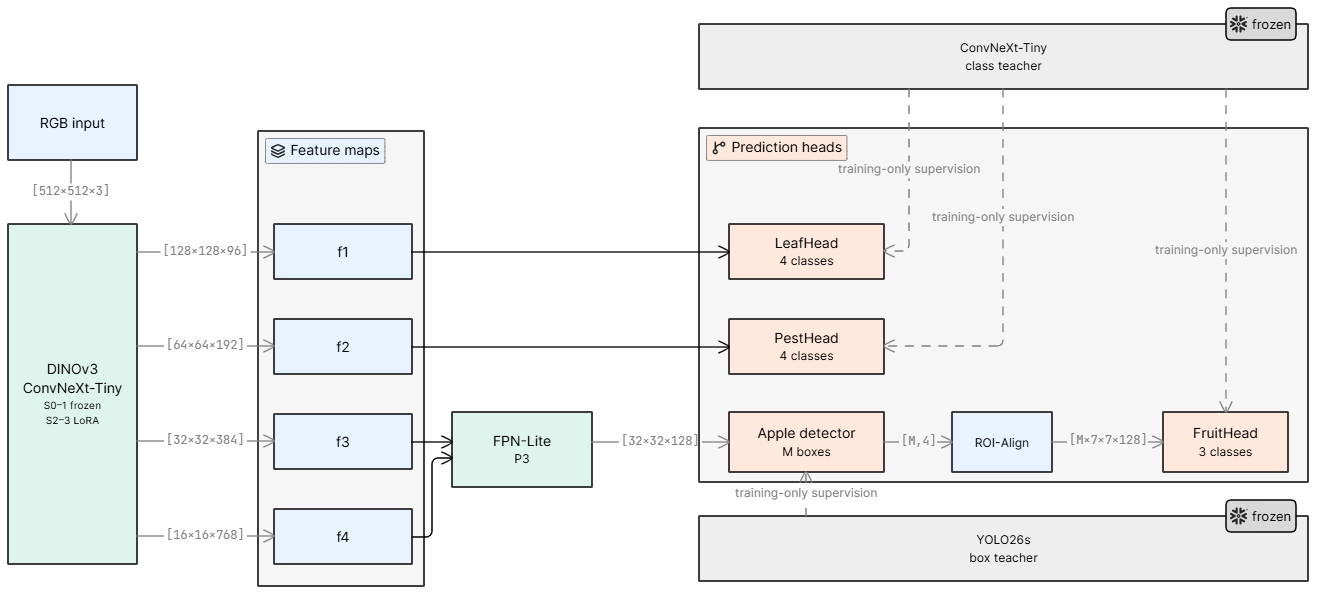
\includegraphics[width=\textwidth]{fig01_architecture.png}
\caption{Unified multi-task architecture. A single shared backbone feeds task-specific heads for leaf disease, pest, fruit grading and apple counting. Solid arrows show offline inference; dashed arrows show training-only teacher supervision detailed in Fig.~\ref{fig:loss}. Schematic; tensor shapes and routing are defined in Eqs.~\ref{eq:features}--\ref{eq:routing-det}.}
\label{fig:arch}
\end{figure}

In Fig.~\ref{fig:arch}, a single $512\times512$ pixel input passes once
through the shared DINOv3-ConvNeXt-Tiny backbone, after which the network
branches by scale rather than by duplicated encoding. Fine-grained stage~1
features carry texture for leaf classification, mid-scale stage~2 features
carry morphology for pest recognition, and the FPN-Lite fusion of stages~3
and 4 carries context for apple detection, from which ROI-Align crops derive
per-apple fruit classification. Solid arrows therefore trace inference, which
is fully shared up to the heads, while dashed arrows trace training-only
teacher supervision formalized in Fig.~\ref{fig:loss} and
Eqs.~\ref{eq:kl}--\ref{eq:yield}. Full stage shapes and routing equalities
appear in Eqs.~\ref{eq:features}--\ref{eq:routing-det}. This scale-to-task
mapping motivates the order of what follows: teachers first, then backbone
and routing, then heads and optimization.

\subsection{Teacher Ensemble}

Specialized teachers provide task supervision. Classification teachers
are ConvNeXt-Small models fine-tuned from a 120-class Plant Disease
Dataset checkpoint (PDDD) [FULL-NAME-AND-SOURCE-TO-BE-INSERTED]. The feature dimension is 768 and dropout is 0.5. Training
uses focal loss with label smoothing 0.1, class-balanced sampling and
heavy augmentation for classes with fewer than 400 training images. It
runs up to 100 epochs with an 8-epoch frozen phase, a 5-epoch warm-up
and cosine warm restarts. Backbone learning rate is $1\times10^{-5}$.
Head learning rate is $1\times10^{-3}$ in phase 1 and
$1\times10^{-4}$ in phase 2.

Three independent classification-teacher seeds are used:
\begin{equation}
S=\{42,123,456\}.
\label{eq:seeds}
\end{equation}

Eight test-time augmentation (TTA) views (original, flips, and
$\pm15^{\circ}$/$\pm30^{\circ}$ rotations) are evaluated per seed.
Consequently, the number of teacher inference passes per image for the
classification soft labels is:
\begin{equation}
N_{\mathrm{TTA}}=3\times 8=24.
\label{eq:tta}
\end{equation}
Per-image soft targets are the TTA mean at temperature~1:
\begin{equation}
P_{T}=\frac{1}{N_{\mathrm{TTA}}}\sum_{k=1}^{N_{\mathrm{TTA}}}P_{T}^{(k)},\quad T=1.
\label{eq:tta-avg}
\end{equation}
The yield task uses a separately trained YOLO26s teacher. Input size
is $640\times640$ pixels with CIELAB enhancement. Confidence threshold is 0.20,
non-maximum suppression (NMS) Intersection over Union (IoU) is 0.45 and the limit is 300 detections per image. Normalized
boxes and scores are stored as soft labels.

\subsection{Categorical and Detection Distillation}

For classification, the TTA-averaged teacher probabilities at
temperature $T=1$ are used directly with no further temperature
scaling. The student matches them through Kullback-Leibler (KL) divergence:
\begin{equation}
L_{\mathrm{KL}}=D_{\mathrm{KL}}(P_{T}\parallel P_{S}),
\label{eq:kl}
\end{equation}
where $P_{T}$ and $P_{S}$ denote teacher and student probability
vectors, averaged over samples whose label differs from the ignore index
$-1$. Hard labels are supervised with focal loss at $\gamma=2.0$,
and the two terms are blended with equal weight:
\begin{equation}
L_{\mathrm{cls}}=\alpha L_{\mathrm{focal}}+(1-\alpha)L_{\mathrm{KL}},\quad \alpha=0.5.
\label{eq:cls}
\end{equation}
Whether this blend helps is tested by the no-distillation ablation,
not assumed.

For detection, supervision is box-level rather than heatmap-based.
Each ground-truth or teacher box with center $(c_{x},c_{y})$ is
assigned to its grid cell:
\begin{equation}
(i,j)=(\lfloor c_{x}W\rfloor,\lfloor c_{y}H\rfloor),\quad W=H=32.
\label{eq:grid}
\end{equation}
At positive cells, box regression uses Complete Intersection over Union (CIoU) loss while
objectness and single-class scores use binary cross-entropy:
\begin{equation}
L_{\mathrm{det}}=\lambda_{\mathrm{box}}L_{\mathrm{CIoU}}+\lambda_{\mathrm{obj}}L_{\mathrm{obj}}+\lambda_{\mathrm{cls}}L_{\mathrm{cls}},
\label{eq:det}
\end{equation}
with:
\begin{equation}
\lambda_{\mathrm{box}}=7.5,\quad \lambda_{\mathrm{obj}}=1.0,\quad \lambda_{\mathrm{cls}}=0.5.
\label{eq:lambdas}
\end{equation}
The loss is computed once against ground-truth boxes and once against
YOLO teacher box coordinates, with the teacher branch scaled
by:
\begin{equation}
L_{\mathrm{yield}}=L_{\mathrm{det}}^{\mathrm{gt}}+\beta L_{\mathrm{det}}^{\mathrm{teacher}},\quad \beta=0.5.
\label{eq:yield}
\end{equation}
The fixed $\beta$ is a stated boundary of the study.

\subsection{Student Backbone and Routing}

The student backbone is DINOv3-ConvNeXt-Tiny via \texttt{timm}
(\texttt{features\_only=True}). For a $512\times512$ pixel input it yields:
\begin{equation}
f1{:}[B,96,128,128],\quad f2{:}[B,192,64,64],\quad f3{:}[B,384,32,32],\quad f4{:}[B,768,16,16].
\label{eq:features}
\end{equation}
Stages 0--1 are fully frozen. Stages 2--3 carry custom LoRA adapters
on \texttt{mlp.fc1}/\texttt{mlp.fc2} with:
\begin{equation}
\mathrm{rank}=8,\quad \alpha=16,\quad \mathrm{dropout}=0.05,
\label{eq:lora}
\end{equation}
all other backbone parameters frozen, leaving only the LoRA $A$/$B$
matrices trainable. The hierarchical routing is:
\begin{equation}
f1\rightarrow \mathrm{Leaf},\quad f2\rightarrow \mathrm{Pest},
\label{eq:routing-cls}
\end{equation}
while $f3$ and $f4$ are fused by the FPN-Lite neck into $P3$:
\begin{equation}
P3=\mathrm{FPN\text{-}Lite}(f3,f4)\in\mathbb{R}^{B\times 128\times 32\times 32}.
\label{eq:fpn}
\end{equation}
The detection and fruit routing from the fused scale is:
\begin{equation}
P3\rightarrow \mathrm{Apple\ Detection},\quad \mathrm{ROIAlign}(P3)\rightarrow \mathrm{Fruit\ Classification}.
\label{eq:routing-det}
\end{equation}
Leaf, pest, and fruit heads predict 4, 4, and 3 classes respectively,
as configured.

\begin{figure}[htbp]
\centering
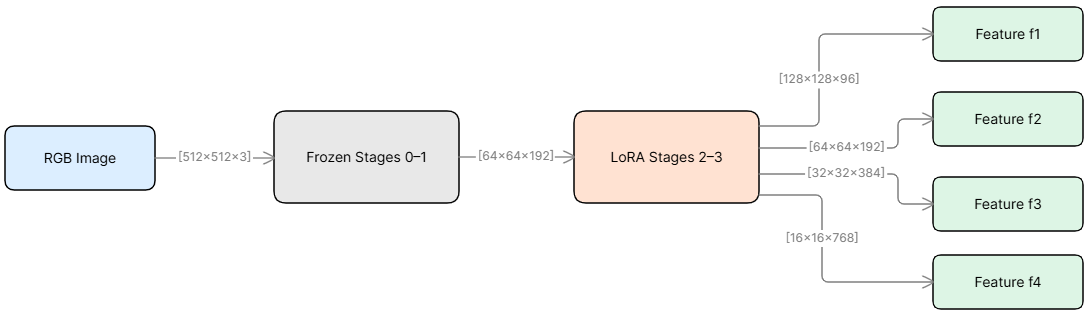
\includegraphics[width=\textwidth]{fig03_routing.png}
\caption{Hierarchical routing from backbone stages to tasks. Stage 1 texture to leaf classification, stage 2 morphology to pest recognition, fused stages 3-4 to apple detection with region of interest Align crops to fruit grading. Schematic; exact tensor shapes are defined in Section~\ref{sec:methodology}.}
\label{fig:routing}
\end{figure}

In Fig.~\ref{fig:routing}, resolution is traded for semantics
along the backbone, and each task taps the scale that matches its visual
cue. Stage~1 retains high-resolution texture essential for leaf lesions,
stage~2 retains mid-resolution shape essential for pest morphology, and the
FPN-Lite fusion in Eq.~\ref{eq:fpn} aggregates deep context essential for
localizing apples under occlusion. Per-apple fruit classification then crops
this fused map with ROI-Align, using ground-truth boxes in training and
decoded boxes in inference, so grading inherits detection geometry rather
than re-encoding the image. The figure thus justifies Eqs.~\ref{eq:features}--\ref{eq:routing-det}
and explains why a single scale cannot serve texture, morphology and
localization at once.

\subsection{Heads, Detection Decoding, and Optimization}

Classification heads share a mobile inverted bottleneck convolution (MBConv) design ($1\times1$ reduction to a
256-channel bottleneck, MBConv block with expansion 4 and squeeze-and-excitation (SE) ratio
0.25, global pooling, dropout $p{=}0.3$, linear classifier) consuming:
\begin{equation}
\mathrm{Leaf}{:}f1\;(96\mathrm{ch})\rightarrow 4,\quad \mathrm{Pest}{:}f2\;(192\mathrm{ch})\rightarrow 4,\quad \mathrm{Fruit}{:}\mathrm{ROI}\;(128\mathrm{ch},7\times7)\rightarrow 3.
\label{eq:heads}
\end{equation}
Detection uses a decoupled anchor-free head on $P3$ emitting:
\begin{equation}
\hat{D}\in\mathbb{R}^{B\times 6\times 32\times 32},
\label{eq:det-head}
\end{equation}
where the six channels are $[c_{x},c_{y},w,h,\mathrm{obj},\mathrm{cls}]$
with sigmoid applied at loss and post-processing time. Decoding keeps
cells with:
\begin{equation}
\mathrm{obj}\times\mathrm{cls}>\mathrm{conf}_{\mathrm{thresh}},\quad \mathrm{conf}_{\mathrm{thresh}}=0.3,
\label{eq:conf}
\end{equation}
followed by non-maximum suppression with:
\begin{equation}
\mathrm{nms}_{\mathrm{iou}}=0.45.
\label{eq:nms}
\end{equation}
Both thresholds match the single operating point used throughout (confidence 0.3 and NMS IoU 0.45; see Experimental Setup).
Per-image counts are decoded boxes. Task balancing uses adaptive weighting based on homoscedastic (task-dependent, input-independent) uncertainty. For task $t$ the weighter maintains:
\begin{equation}
s_{t}=\log(\sigma_{t}^{2}),\quad \mathrm{initialized\ to\ }0.
\label{eq:logvar}
\end{equation}
The multi-task objective is:
\begin{equation}
L_{\mathrm{MTL}}=\sum_{t\in\mathcal{T}}\left(e^{-s_{t}}L_{t}+\frac{1}{2}s_{t}\right),
\label{eq:mtl}
\end{equation}
where:
\begin{equation}
\mathcal{T}=\{\mathrm{leaf},\mathrm{pest},\mathrm{fruit},\mathrm{yield}\}.
\label{eq:tasks}
\end{equation}
No hard clamping is imposed on $s_{t}$; reported weights are precisions:
\begin{equation}
w_{t}=e^{-s_{t}}.
\label{eq:tweight}
\end{equation}
Distillation needs no extra global coefficients because
it is contained inside per-task losses ($\alpha$ in Eq.~\ref{eq:cls},
$\beta$ in Eq.~\ref{eq:yield}). Hence:
\begin{equation}
L_{\mathrm{total}}=L_{\mathrm{MTL}}.
\label{eq:total}
\end{equation}
Training is two-phase with 5 epochs for heads and neck with low-rank adaptation (LoRA) frozen,
then LoRA at $10^{-5}$ against heads at $10^{-4}$ with AdamW, cosine schedule,
accumulation $\times4$, clip 1.0, patience 20 and automatic mixed precision (AMP) off; the static-weight
ablation replaces the weighter with a plain sum.

\begin{figure}[htbp]
\centering
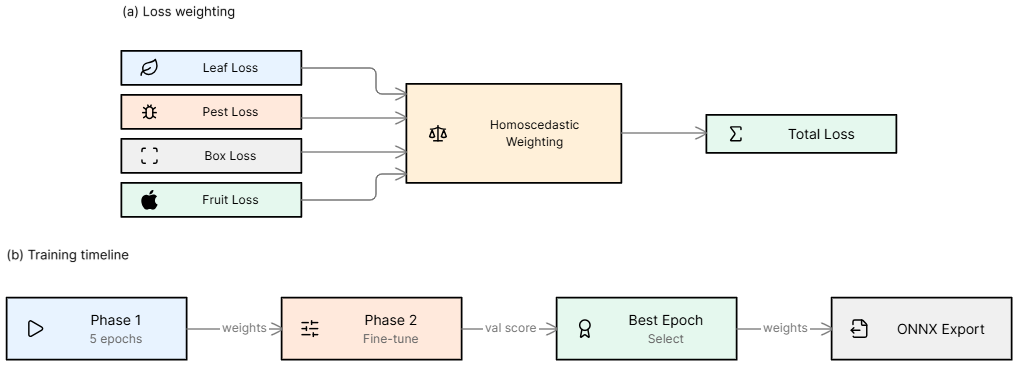
\includegraphics[width=\textwidth]{fig04_loss_training.png}
\caption{Heterogeneous distillation and two-phase training. \textbf{a}, classification supervision from test-time augmentation-averaged soft targets and detection supervision from teacher boxes. \textbf{b}, training timeline with head-only warm-up, joint LoRA adaptation, best validation at epochs 186 and 194, and Open Neural Network Exchange export. Schematic; loss definitions are in Eqs.~\ref{eq:kl}--\ref{eq:total}.}
\label{fig:loss}
\end{figure}

In Fig.~\ref{fig:loss}, panel~a separates the two teacher
streams that supervise one student: TTA-averaged soft targets distil
category knowledge into the leaf, pest and fruit heads through
Eqs.~\ref{eq:kl}--\ref{eq:cls}, while YOLO boxes distil spatial knowledge
into the detection grid through Eqs.~\ref{eq:grid}--\ref{eq:yield}. Data
thus flow forward through routing while gradients flow backward from
heterogeneous teachers. Panel~b places this supervision on a two-phase
timeline, with head-only warm-up before joint LoRA adaptation, best
validation at epochs 186 and 194, and ONNX export closing training. The
figure therefore links Fig.~\ref{fig:arch} to Eqs.~\ref{eq:seeds}--\ref{eq:total}
and hands over to data and measurement next.

\FloatBarrier
\section{Dataset Curation and Preprocessing}
\label{sec:dataset}

The methodology requires clean, stratified inputs before any loss in
Eqs.~\ref{eq:kl}--\ref{eq:total} can be trusted. This section therefore
quantifies what the teachers in Section~\ref{sec:methodology} actually
saw, so that ceiling effects reported in Section~\ref{sec:results} are
traceable to data rather than speculation.

Leaf images come from a public PlantVillage mirror on
Kaggle~\cite{leafkaggle} [LICENSE-AND-ACCESSED-DATE-TO-BE-INSERTED], of which only the apple leaf classes relevant
to the four-class leaf task are used. Fruit images combine a Kaggle apple
fruit disease collection~\cite{fruitkaggle} [LICENSE-AND-ACCESSED-DATE-TO-BE-INSERTED] with a Mendeley apple fruit
dataset, version 6~\cite{fruitmendeley}, restricted to the Anthracnose,
Black Rot and Healthy classes of Table~\ref{tab:dataset}. Pest images come
from a Kaggle apple leaf and fruit disease segmentation
collection~\cite{pestkaggle} [LICENSE-AND-ACCESSED-DATE-TO-BE-INSERTED], restricted to the four pest classes evaluated
here. Apple detection images come from a Kaggle apple quality
collection~\cite{applequality} [LICENSE-AND-ACCESSED-DATE-TO-BE-INSERTED]. No repository is used in full; each
contributes only its project-relevant subset, and the Raw column of
Table~\ref{tab:dataset} reports post-subset, pre-cleaning totals for the
classification tasks. Full links, licenses and access dates are listed in Data Availability; third-party images are not redistributed.

All classification images pass through automated cleaning: images
smaller than $64$ pixels on the shortest side or with pixel standard deviation below $5.0$ are
removed, with perceptual-hash deduplication at Hamming threshold 8 [LIBRARY-VERSION-TO-BE-INSERTED]. Table~\ref{tab:dataset} shows retained counts per class remain sufficient
for stratified learning. The largest absolute drops are Leaf Healthy from
2276 to 2152 and Fruit Healthy from 1424 to 1333 after duplicate removal,
while minority classes such as Pest aphids from 314 to 270 and Fruit
Anthracnose from 295 to 275 lose only tens of images. Cleaning is therefore
mild and balanced rather than destructive, so the stratified sampling that
follows preserves class ratios instead of amplifying imbalance.

\begin{table}[t]
\centering
\caption{Teacher-side dataset cleaning (raw $\rightarrow$ clean).}
\label{tab:dataset}
\begin{tabular}{lcc}
\toprule
\textbf{Class} & \textbf{Raw} & \textbf{Clean} \\
\midrule
Leaf: Apple\_Mosaic & 631 & 622 \\
Leaf: Apple\_\_\_Black\_rot & 621 & 579 \\
Leaf: Alternaria & 631 & 621 \\
Leaf: Healthy & 2276 & 2152 \\
\midrule
Pest: xylotrechus & 319 & 296 \\
Pest: aphids & 314 & 270 \\
Pest: leafhoppers & 573 & 567 \\
Pest: spider\_mite & 299 & 271 \\
\midrule
Fruit: Anthracnose & 295 & 275 \\
Fruit: Black Rot & 542 & 524 \\
Fruit: Healthy & 1424 & 1333 \\
\bottomrule
\end{tabular}
\end{table}

Each classification task uses stratified 70/15/15 train/val/test splits
with seed 42; yield detection uses its own split of 1093 train and 264 val.
Inputs are $224\times224$ pixels for classification teachers,
$640\times640$ pixels for the YOLO26s teacher, and $512\times512$ pixels for the
student. Two boundary facts matter later: leaf and pest validation sit
near ceiling because teachers are saturated, and no Healthy fruit region of interest (ROI)
survives into validation or test.

Segmentation and box labels for apple fruits did not pre-exist and were
produced semi-automatically: candidate masks were generated with the base
Segment Anything Model (SAM) from Meta~\cite{sam2023} [VERSION-TO-BE-INSERTED] inside
X-AnyLabeling~\cite{xanylabeling2023} [VERSION-TO-BE-INSERTED], operated manually by the authors, for apple fruits
only. Every image was then manually verified before use [VERIFIER-INITIALS-AND-PROTOCOL-TO-BE-INSERTED], so no SAM
proposal enters training or evaluation unverified. Classification labels
for leaf, pest and fruit were used as provided by their sources.

\begin{figure}[htbp]
\centering
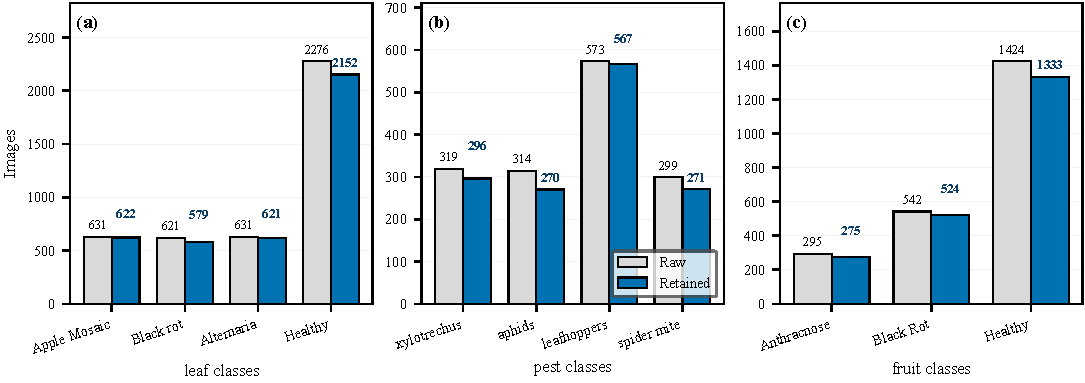
\includegraphics[width=\textwidth]{fig02_dataset}
\caption{Dataset curation pipeline. Cleaning, perceptual-hash deduplication and stratified 70/15/15 splits for leaf, pest and fruit teachers; yield detection uses its own 1093 train and 264 validation split. Class counts before and after cleaning are in Table~\ref{tab:dataset}. Schematic.}
\label{fig:dataset}
\end{figure}

Fig.~\ref{fig:dataset} summarizes the curation pipeline, which applies the
same cleaning, deduplication and stratified splitting to leaf, pest and
fruit teachers, while yield follows a separate detection split. Corrupt
and near-duplicate images are removed without collapsing any minority
class, so the class histograms before and after cleaning retain their
shape. The distribution is therefore preserved for the class-balanced
sampling and heavy augmentation of rare classes described in
Section~\ref{sec:methodology}, which explains why later ceiling effects
can be attributed to task difficulty rather than to data loss.

\FloatBarrier
\section{Experimental Setup}
\label{sec:experimental}

With data (Section~\ref{sec:dataset}) and model (Section~\ref{sec:methodology})
fixed, this section fixes how measurement is done: implementation,
optimization hyperparameters, and metric definitions in
Eqs.~\ref{eq:acc}--\ref{eq:rmse}. Every number in
Section~\ref{sec:results} is produced under exactly this protocol, so
no result appears without a preceding definition.

The framework is implemented in PyTorch with \texttt{timm} backbones,
Albumentations and scikit-learn [VERSIONS-TO-BE-INSERTED; see Code Availability for repository link and commit hash],
with Open Neural Network Exchange (ONNX) export at opset 17 of leaf
logits, pest logits, and the raw detection grid; fruit runs
client-side from region of interest Align (ROI-Align) crops. Students train up to 200 epochs
with batch 8 and accumulation $\times4$ for effective 32 on RTX A4000-class
GPU, with automatic mixed precision (AMP) off since Complete Intersection over Union (CIoU) and Kullback-Leibler (KL) terms proved unstable in FP16, with AdamW at
weight decay $10^{-4}$, low-rank adaptation (LoRA) $10^{-5}$ and heads, neck and weighter $10^{-4}$,
cosine annealing to $\eta_{min}{=}10^{-7}$, clipping at norm 1.0, and
early stopping with patience 20 and min-delta $10^{-4}$ on total validation
loss.

Classification accuracy is:
\begin{equation}
\mathrm{Accuracy}=\frac{N_{\mathrm{correct}}}{N_{\mathrm{total}}}.
\label{eq:acc}
\end{equation}
Class-wise precision, recall, and F1-score are:
\begin{equation}
\mathrm{Precision}=\frac{TP}{TP+FP},
\label{eq:prec}
\end{equation}
\begin{equation}
\mathrm{Recall}=\frac{TP}{TP+FN},
\label{eq:rec}
\end{equation}
\begin{equation}
F1=2\frac{\mathrm{Precision}\times\mathrm{Recall}}{\mathrm{Precision}+\mathrm{Recall}}.
\label{eq:f1}
\end{equation}
For fruit counting over $M$ images with predicted $\hat{N}_{j}$ and
ground-truth $N_{j}$ counts:
\begin{equation}
\mathrm{MAE}=\frac{1}{M}\sum_{j=1}^{M}|\hat{N}_{j}-N_{j}|,
\label{eq:mae}
\end{equation}
\begin{equation}
\mathrm{RMSE}=\sqrt{\frac{1}{M}\sum_{j=1}^{M}(\hat{N}_{j}-N_{j})^{2}}.
\label{eq:rmse}
\end{equation}
Counting uses decoded boxes at the operating point defined here,
namely confidence 0.3 and non-maximum suppression (NMS) Intersection over Union (IoU) 0.45. Unless stated otherwise, all
detection results use this operating point. All runs use a single seed
and early stopping with patience 20. Best epochs are selected by total
validation loss. No confidence intervals or P values are computed; this single-seed limitation is stated as a limitation.

\FloatBarrier
\section{Results}
\label{sec:results}
%% SCI REP DISPLAY PLAN (limit 8 figs+tables for typesetting; excess to Supplementary on revision):
%% Keep in main: Fig arch, Fig results overall, Fig ablation, Fig confusion, Fig counting,
%% Fig boxes, Fig edge + 1-2 tables. Move to Supplementary: routing, loss timeline,
%% dataset schematic, frozen-vs-proposed deltas, convergence, weights, per-class tables,
%% confidence maps. Science unchanged; only placement changes.

Results are presented in the order the methodology promised:
overall reference, frozen control, convergence check, weight
inspection, ablation verdict, per-class diagnosis, counting diagnosis,
and on-device proof. Each subsection cites its table and figure pair
explicitly, and each closes by stating what the next subsection must
explain, so the chapter reads as one argument rather than isolated
snapshots.

\subsection{Overall Performance}

The proposed Agri-CNX-Edge model is the reference that later ablations take apart (single run per configuration; differences of less than about 3 percentage points on fruit are within estimated run-to-run variation and are reported without confidence intervals or P values).
Table~\ref{tab:final_results} gives best-validation accuracy of
99.67\% for leaf, 100.00\% for pest and 96.30\% for fruit, with counting
MAE 3.5675 and RMSE 6.3767 on 400 yield images. The table thus separates
two regimes: leaf and pest sit at ceiling where further gains are
numerically impossible, while fruit accuracy trails by nearly four points
and counting errors remain well above zero. In Fig.~\ref{fig:final},
the accuracy panel makes this split visual by placing leaf and pest bars at
the top of the scale against a distinctly lower fruit bar, while the error
panel places MAE and RMSE on a count scale that exposes the spatial task as
the remaining challenge. Together, table values and figure shapes establish
where diagnosis must focus. Leaf and pest therefore offer no further signal,
so the next subsection turns to fruit and counting.

\begin{table}[t]
\centering
\caption{Best-validation performance of the proposed model.}
\label{tab:final_results}
\begin{tabular}{lcc}
\toprule
\textbf{Task} & \textbf{Metric} & \textbf{Performance} \\
\midrule
Leaf disease classification & Accuracy (val) & 99.67\% \\
Pest recognition & Accuracy (val) & 100.00\% \\
Fruit classification & Accuracy (val) & 96.30\% \\
Fruit localization/counting & Count MAE & 3.5675 \\
Fruit localization/counting & Count RMSE & 6.3767 \\
\bottomrule
\end{tabular}
\end{table}

\begin{figure}[htbp]
\centering
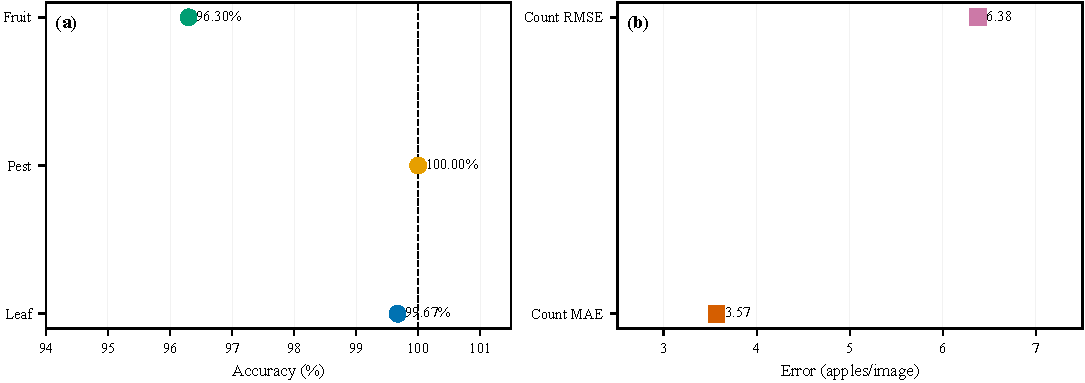
\includegraphics[width=\textwidth]{fig05_final_performance}
\caption{Best-validation performance of the proposed model. Accuracies for leaf, pest and fruit classification and counting errors for yield. Validation sample sizes are defined in Section~\ref{sec:dataset}; counting errors are on 400 yield images. Bars show point estimates from a single run without error bars.}
\label{fig:final}
\end{figure}

\subsection{Frozen Versus Proposed Configuration}

Checkpoint inspection confirms attribution, as low-rank adaptation (LoRA) adapters are present
only in the proposed checkpoint. Table~\ref{tab:frozen_proposed} shows adaptation improves leaf marginally
from 99.50\% to 99.67\%, a gain of 0.17 points, and holds pest equal at
100.00\%, but reduces fruit accuracy from 98.42\% to 96.30\%, a loss of
2.12 points, while increasing counting error from MAE 3.4300 to 3.5675
and RMSE 6.0017 to 6.3767. The table therefore documents an inversion:
the only task that improves is already at ceiling, while the headroom
tasks of fruit grading and dense localization degrade. Paired deltas in Fig.~\ref{fig:compare}
visualize the same inversion, with a near-zero leaf bar
against clearly negative fruit and counting bars. The pattern is reported
as observed rather than rationalized, and it motivates the full ablation
that isolates adaptation, distillation, weighting and warm-up.

\begin{table}[t]
\centering
\caption{Frozen and proposed configurations with paired deltas.}
\label{tab:frozen_proposed}
\begin{tabular}{lccc}
\toprule
\textbf{Metric} & \textbf{Frozen} & \textbf{Proposed} & \textbf{Change} \\
\midrule
Leaf Accuracy & 99.50\% & 99.67\% & +0.17 pp \\
Pest Accuracy & 100.00\% & 100.00\% & 0.00 pp \\
Fruit Accuracy & 98.42\% & 96.30\% & -2.12 pp \\
Count MAE & 3.4300 & 3.5675 & +0.1375 \\
Count RMSE & 6.0017 & 6.3767 & +0.3750 \\
\bottomrule
\end{tabular}
\end{table}

\begin{figure}[htbp]
\centering
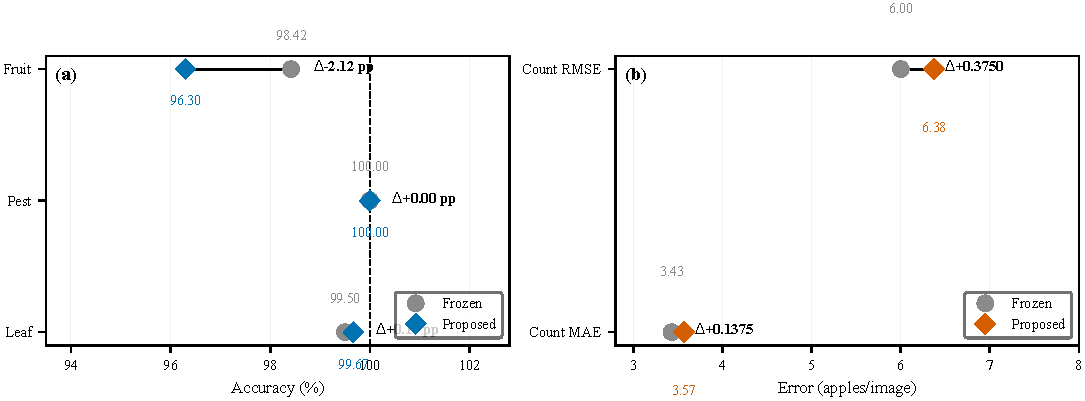
\includegraphics[width=\textwidth]{fig06_frozen_vs_proposed}
\caption{Frozen and proposed configurations with paired deltas.}
\label{fig:compare}
\end{figure}

\subsection{Training Convergence}

Convergence timing does not explain the fruit gap. Table~\ref{tab:convergence} gives best epochs are 186 for the proposed run and
194 for the frozen run, with best validation losses of $-$1.9251 and
$-$1.9271 and training losses of $-$0.7437 and $-$0.6637 at those epochs.
Both the timing and the loss levels are near identical, so neither
under-training nor overfitting distinguishes the two runs. In
Fig.~\ref{fig:conv}, panel~a shows overlapping training and validation
loss trajectories across 200 epochs, while panel~b shows per-task
validation accuracy in which leaf and pest flatten early near 100\%
and fruit oscillates most across epochs. The visual message matches the
tabular one: optimization length is not the bottleneck. The cause must
therefore lie in task weighting rather than training length, which leads
to the next subsection.

\begin{table}[t]
\centering
\caption{Training convergence at best-validation epochs.}
\label{tab:convergence}
\begin{tabular}{lcc}
\toprule
\textbf{Training Statistic} & \textbf{Proposed} & \textbf{Frozen}\\
\midrule
Best epoch & 186 & 194\\
Best validation loss & -1.9251 & -1.9271\\
Training loss at best epoch & -0.7437 & -0.6637\\
\bottomrule
\end{tabular}
\end{table}

\begin{figure}[htbp]
\centering
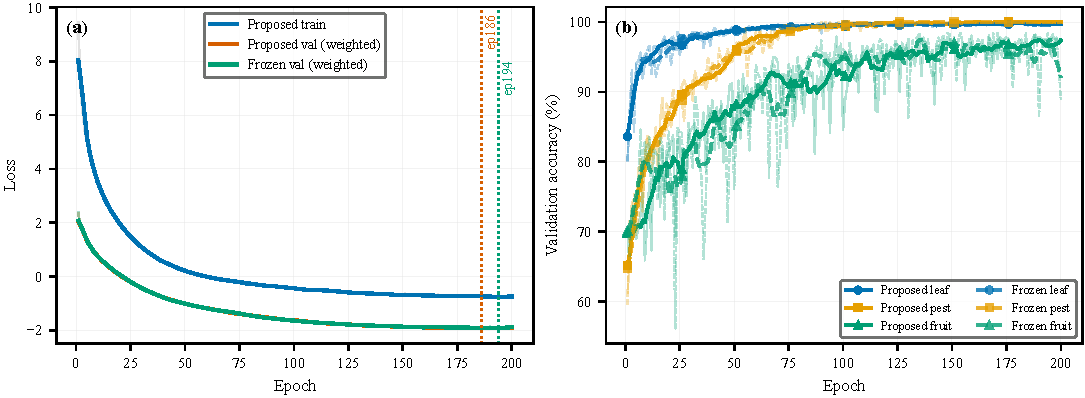
\includegraphics[width=\textwidth]{fig07_convergence}
\caption{Training dynamics over 200 epochs. Panel a shows training and
validation loss. Panel b shows per-task validation accuracy.}
\label{fig:conv}
\end{figure}

\subsection{Learned Task Weights}

Learned precisions in Eq.~\ref{eq:tweight} are optimization coefficients
rather than measures of importance. Tables~\ref{tab:weights_proposed} and
\ref{tab:weights_frozen} and Fig.~\ref{fig:weights} show fruit receives
the largest weight in both runs, 18.8170 for the proposed run at epoch 186
and 18.4710 for the frozen run at epoch 194, followed by leaf at 6.9591 and
7.1471, pest at 5.7344 and 5.7203, and yield at 0.1780 and 0.1760, with
nearly identical ordering across runs. The figure makes this hierarchy
immediate by placing the fruit bar far above the rest in both runs, while
the tables supply the exact precisions. Such stability across adaptation
states shows that the weighting reflects loss scale rather than task
priority. Whether this learned balance matters is tested by replacing it
with equal weights in the ablation.

\begin{table}[t]
\centering
\caption{Terminal task precisions, proposed (epoch 186).}
\label{tab:weights_proposed}
\begin{tabular}{lc}
\toprule
\textbf{Task} & \textbf{Terminal Weight}\\
\midrule
Fruit & 18.8170\\
Leaf & 6.9591\\
Pest & 5.7344\\
Yield & 0.1780\\
\bottomrule
\end{tabular}
\end{table}

\begin{table}[t]
\centering
\caption{Terminal task precisions, frozen (epoch 194).}
\label{tab:weights_frozen}
\begin{tabular}{lc}
\toprule
\textbf{Task} & \textbf{Terminal Weight}\\
\midrule
Fruit & 18.4710\\
Leaf & 7.1471\\
Pest & 5.7203\\
Yield & 0.1760\\
\bottomrule
\end{tabular}
\end{table}

\begin{figure}[htbp]
\centering
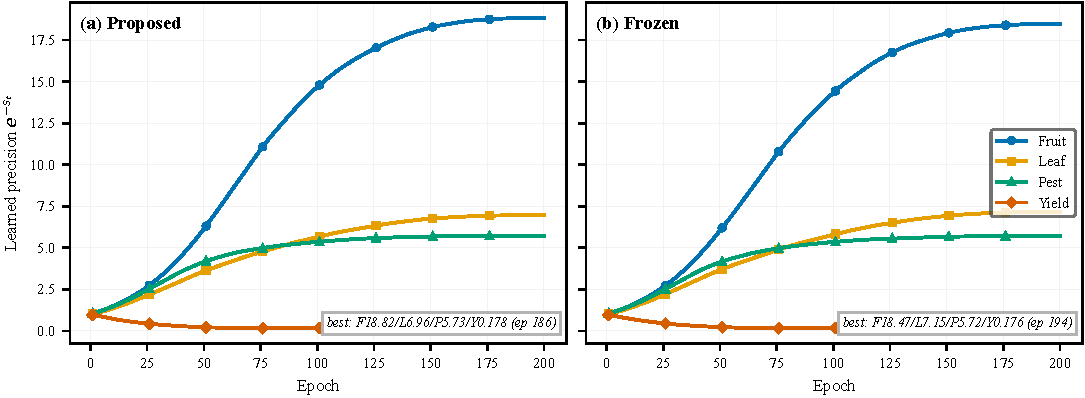
\includegraphics[width=\textwidth]{fig08_task_weights}
\caption{Learned task precisions for proposed and frozen runs. Terminal weights at best-validation epochs 186 and 194; fruit receives the largest weight in both runs. Single run; weights are optimization coefficients, not importance measures.}
\label{fig:weights}
\end{figure}

\FloatBarrier
\section{Ablation Study}
\label{sec:ablation}

Each configuration removes one component while holding the rest fixed.
Table~\ref{tab:ablation} reports best-validation epochs:
removing distillation without knowledge distillation (KD) matches or improves every validation metric,
with leaf rising from 99.67\% to 100.00\%, pest holding at 100.00\%, fruit
rising from 96.30\% to 98.47\%, MAE falling from 3.5675 to 3.0175 and RMSE
falling from 6.3767 to 5.2714, while replacing learned weighting with equal
weights collapses validation fruit to 81.43\%. On held-out test the same
ranking holds and widens: without KD reaches 99.14\% fruit with MAE 3.08
against proposed 95.69\% with MAE 3.53, while static weighting falls further
to 70.26\% fruit. Adaptation without low-rank adaptation (LoRA) at 94.69\% and without warm-up at
97.18\% remain within run-to-run noise. In Fig.~\ref{fig:ablation},
the radar makes the ranking visual by enclosing the largest area for the
no-distillation run and the smallest for static weighting, with the exact
values tabulated alongside. The static-weighting run stopped after 103 epochs
and is therefore flagged as incomplete, which Section~\ref{sec:limitations} revisits. All values are single runs without confidence intervals or P values.

\begin{table}[t]
\centering
\caption{Component ablation at best-validation epochs. Single run per configuration without confidence intervals or P values. Static weighting
is incomplete at 103 epochs and is interpreted only as collapse evidence.}
\label{tab:ablation}
\begin{tabular}{lccccc}
\toprule
\textbf{Config} & \textbf{Leaf} & \textbf{Pest} & \textbf{Fruit} &
\textbf{MAE} & \textbf{RMSE} \\
\midrule
Proposed & 99.67\% & 100.00\% & 96.30\% & 3.5675 & 6.3767 \\
No KD & 100.00\% & 100.00\% & 98.47\% & 3.0175 & 5.2714 \\
Static & 99.35\% & 98.33\% & 81.43\% & 3.5825 & 6.0640 \\
No LoRA & 99.67\% & 99.58\% & 94.69\% & 3.6300 & 6.2032 \\
No warm-up & 99.67\% & 100.00\% & 97.18\% & 3.6575 & 6.6695 \\
Frozen & 99.50\% & 100.00\% & 98.42\% & 3.4300 & 6.0017 \\
\bottomrule
\end{tabular}
\end{table}

\begin{figure}[htbp]
\centering
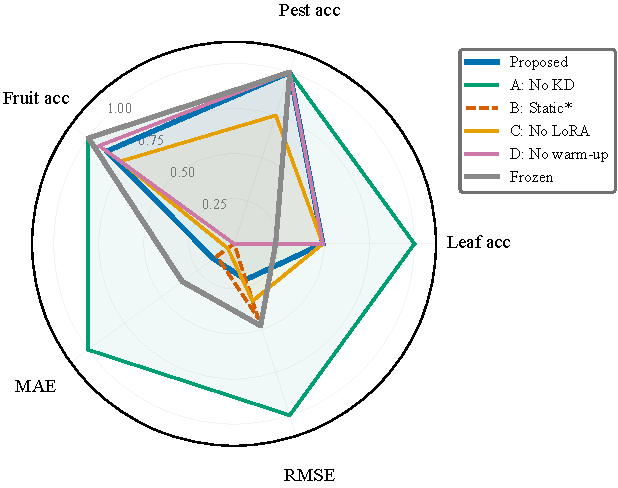
\includegraphics[width=\textwidth]{fig09_ablation}
\caption{Component ablation ranking. Radar encloses the largest area for the no-distillation run and the smallest for static weighting; exact best-validation values are tabulated alongside. Single run per configuration.}
\label{fig:ablation}
\end{figure}

\FloatBarrier
\section{Class-wise Classification Analysis}
\label{sec:classwise}

The following subsections move from validation to held-out test. Leaf
and pest confirm ceiling behavior while fruit reveals headroom. Each
pair of figure and table tells one story, with the figure showing error
location and the table quantifying it.

\subsection{Leaf Disease Classification}

Held-out predictions on 623 images give a clean sweep. The evaluation
uses the latest checkpoint because only it was present on the test
machine, as noted in Section~\ref{sec:limitations}. Fig.~\ref{fig:confusion}a and Table~\ref{tab:leaf_classwise} show the confusion
matrix is perfectly diagonal with zero off-diagonal entries, and all four
classes reach precision, recall and F1-score of 1.0000. Such perfection across
Apple Mosaic, Black rot, Alternaria and Healthy confirms that texture cues
from stage~1 are fully sufficient. Leaf is therefore at ceiling, consistent
with the 99.67\% validation accuracy, and needs no further diagnosis.

\begin{figure}[htbp]
\centering
\begin{minipage}{0.32\textwidth}
\centering
\textbf{a}\par
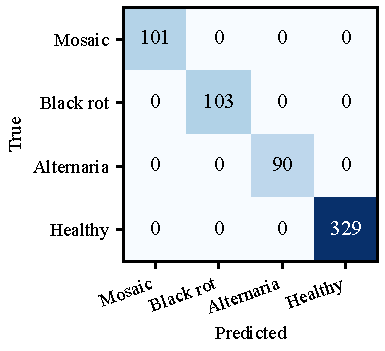
\includegraphics[width=\linewidth]{fig10_leaf_cm_c}
\end{minipage}\hfill
\begin{minipage}{0.32\textwidth}
\centering
\textbf{b}\par
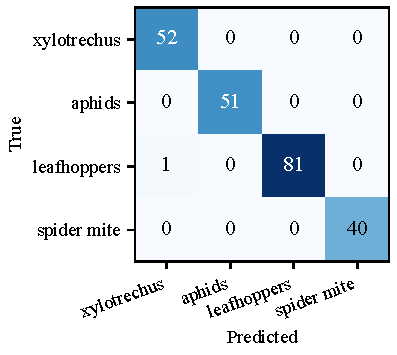
\includegraphics[width=\linewidth]{fig11_pest_cm_c}
\end{minipage}\hfill
\begin{minipage}{0.32\textwidth}
\centering
\textbf{c}\par
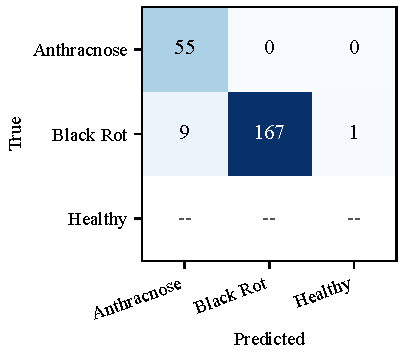
\includegraphics[width=\linewidth]{fig12_fruit_cm_c}
\end{minipage}
\caption{Confusion matrices on held-out test. \textbf{a}, leaf disease on 623 images, perfectly diagonal. \textbf{b}, pest recognition on 225 images with one leafhoppers to xylotrechus error. \textbf{c}, fruit grading on ground-truth regions of interest with no Healthy cases, errors concentrated between Black Rot and Anthracnose. Point estimates from a single run.}
\label{fig:confusion}
\end{figure}

\begin{table}[htbp]
\centering
\caption{Leaf test results by class on 623 held-out images. Single run with the latest checkpoint, not the best-validation epoch.}
\label{tab:leaf_classwise}
\begin{tabular}{lccc}
\toprule
\textbf{Class} & \textbf{Precision} & \textbf{Recall} & \textbf{F1} \\
\midrule
Apple\_Mosaic & 1.0000 & 1.0000 & 1.0000\\
Apple\_\_\_Black\_rot & 1.0000 & 1.0000 & 1.0000\\
Alternaria & 1.0000 & 1.0000 & 1.0000\\
Healthy & 1.0000 & 1.0000 & 1.0000\\
\bottomrule
\end{tabular}
\end{table}

\subsection{Pest Recognition}

One error occurs in 225 test images. Fig.~\ref{fig:confusion}b
and Table~\ref{tab:pest_classwise} show a single leafhoppers image is
predicted as xylotrechus, which lowers xylotrechus precision to 0.9811 and
leafhoppers recall to 0.9878, with corresponding F1-score of 0.9905 and 0.9939,
while aphids and spider mite remain perfect at 1.0000. The confusion matrix
is therefore diagonal except for one cell, consistent with visual similarity
between small insects rather than systematic failure.
Pest is thus also at ceiling at 99.56\% test accuracy, matching validation.

\begin{table}[htbp]
\centering
\caption{Pest test results by class on 225 held-out images. Single run.}
\label{tab:pest_classwise}
\begin{tabular}{lccc}
\toprule
\textbf{Class} & \textbf{Precision} & \textbf{Recall} & \textbf{F1} \\
\midrule
xylotrechus & 0.9811 & 1.0000 & 0.9905\\
aphids & 1.0000 & 1.0000 & 1.0000\\
leafhoppers & 1.0000 & 0.9878 & 0.9939\\
spider\_mite & 1.0000 & 1.0000 & 1.0000\\
\bottomrule
\end{tabular}
\end{table}

\subsection{Fruit Classification}

Fruit is evaluated as a head diagnostic on ground-truth regions of interest (ROIs). No
Healthy ROI exists in validation or test, so generalization for that
class remains untested. Fig.~\ref{fig:confusion}c and
Table~\ref{tab:fruit_classwise} show Anthracnose reaches recall 1.0000 but
precision only 0.8594 with F1-score 0.9244, while Black Rot reaches precision
1.0000 but recall only 0.9435 with F1-score 0.9709, so confusion concentrates
between Black Rot and Anthracnose in one direction. This asymmetry defines
fruit at 95.69\% test accuracy as the headroom task. It links back to the
validation gap of 96.30\% and forward to counting, which shares the same
fused features.

\begin{table}[htbp]
\centering
\caption{Fruit region-of-interest test results by class on ground-truth regions. Healthy has no test regions; single run.}
\label{tab:fruit_classwise}
\begin{tabular}{lccc}
\toprule
\textbf{Class} & \textbf{Precision} & \textbf{Recall} & \textbf{F1} \\
\midrule
Anthracnose & 0.8594 & 1.0000 & 0.9244\\
Black Rot & 1.0000 & 0.9435 & 0.9709\\
Healthy & --- & --- & ---\\
\bottomrule
\end{tabular}
\end{table}

\FloatBarrier
\section{Fruit Counting and Spatial Evaluation}
\label{sec:counting}

Counting correlates well but undercounts systematically on dense
clusters. Table~\ref{tab:counting} gives, on 400 yield images, MAE
3.5300 and RMSE 6.1323 with Pearson $r{=}0.8508$ and $R^{2}{=}0.5700$,
while mean signed error is $-$3.1000. High correlation with negative bias
thus separates ranking quality from systematic undercounting: the model
orders images correctly yet predicts too few apples per image. In
Fig.~\ref{fig:counting}, predictions cluster below the identity line with
widening spread at high counts, so sparse orchard images lie near the line
while dense clusters fall clearly beneath it, visualizing the same bias
numerically reported in the table.

\begin{table}[t]
\centering
\caption{Counting performance on 400 yield images at confidence 0.3 and non-maximum suppression IoU 0.45. Single run without confidence intervals or P values.}
\label{tab:counting}
\begin{tabular}{lc}
\toprule
\textbf{Metric} & \textbf{Value}\\
\midrule
Count MAE & 3.5300\\
Count RMSE & 6.1323\\
Pearson correlation & 0.8508\\
$R^2$ & 0.5700\\
Mean signed error & -3.1000\\
\bottomrule
\end{tabular}
\end{table}

\begin{figure}[htbp]
\centering
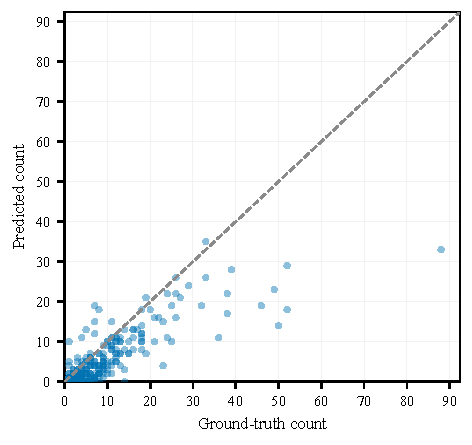
\includegraphics[width=\columnwidth]{fig13_counting}
\caption{Fruit counting accuracy on 400 yield images. Predicted counts versus ground-truth counts with identity reference. Points below the line show systematic undercounting in dense clusters. Single run at confidence 0.3 and non-maximum suppression IoU 0.45; mean absolute error 3.53, root mean square error 6.13, Pearson r 0.85 and R-squared 0.57 without confidence intervals.}
\label{fig:counting}
\end{figure}

Fig.~\ref{fig:boxes} shows sparse cases with one to five apples
match ground truth exactly, while dense clusters with overlapping canopies
miss occluded instances, which is the spatial counterpart of the $-$3.1 bias
in Table~\ref{tab:counting}. In
Fig.~\ref{fig:qualitative}, detector confidence maps are sharp on isolated
apples and decay in clutter, so missed detections coincide with low
confidence regions rather than with random error. These figures complete the
spatial half of the claim opened in Fig.~\ref{fig:arch} and point to
threshold calibration for dense scenes as the natural remedy.

\begin{figure}[htbp]
\centering
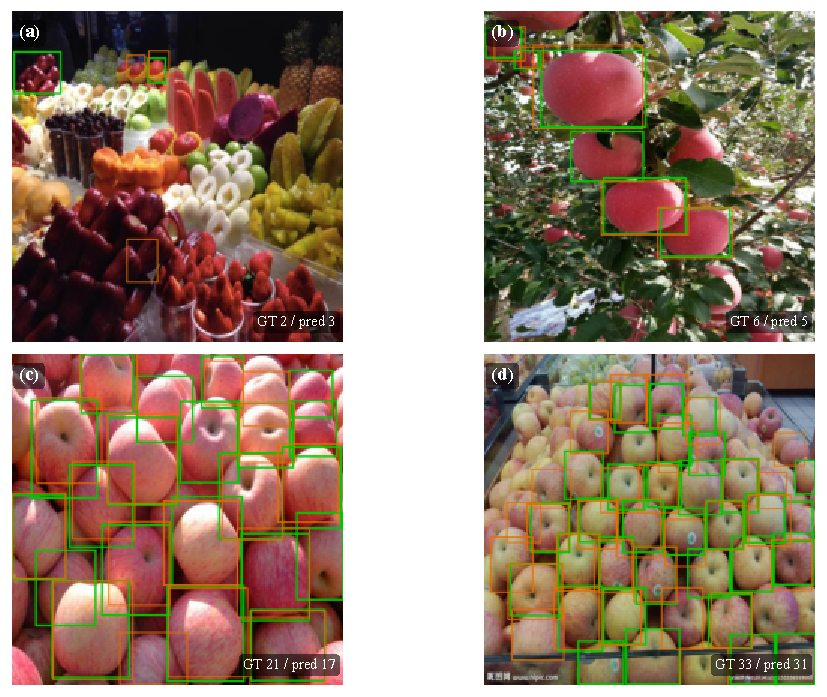
\includegraphics[width=\textwidth]{fig14_boxes}
\caption{Detected boxes from sparse to dense cases. Ground-truth and predicted boxes with per-image counts at confidence 0.3 and non-maximum suppression IoU 0.45. Sparse cases with one to five apples match exactly; dense overlapping canopies miss occluded instances. Single run.}
\label{fig:boxes}
\end{figure}

\begin{figure}[htbp]
\centering
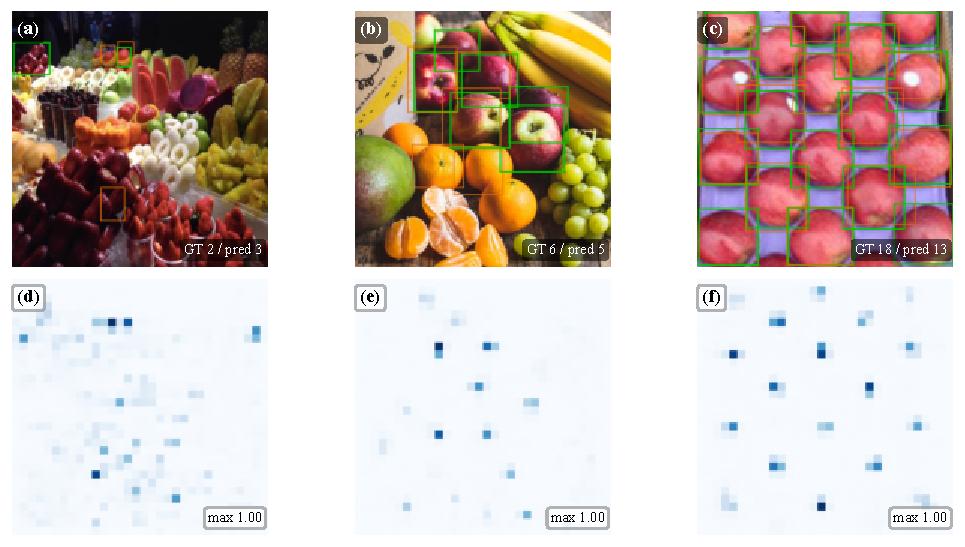
\includegraphics[width=\textwidth]{fig15_qualitative}
\caption{Detector confidence maps for sparse and dense cases. Inputs with counts and corresponding confidence maps. Maps are sharp on isolated apples and decay in clutter where detections are missed. Single run at the same operating point.}
\label{fig:qualitative}
\end{figure}

\FloatBarrier
\section{Edge Deployment Analysis}
\label{sec:edge}

Shared computation must be measured rather than asserted. Tests use a
Samsung A17 5G with ONNX Runtime (ORT) under a uniform protocol with an
accuracy pass over 30 yield and 20 pest images and a latency pass over 100
measured plus 10 warm-up inferences per mode using CPU and
Neural Networks API (NNAPI) providers, using the same app, model,
images and code in both provider modes. Full protocol details are in the
accompanying benchmark description. Table~\ref{tab:edge} shows the unified 120.7\,MB student with 28.28\,M parameters
including 0.46\,M low-rank adaptation (LoRA) is substantially smaller than the teachers at
188.8, 188.8 and 19.4\,MB, phone yield MAE is 2.9 for both CPU and NNAPI over
30 images with 20 of 20 pest agreement to laptop in both modes and zero
CPU to NNAPI prediction differences. Mean latency is 5749\,ms for CPU and
5604\,ms for NNAPI, with p50 of 7041 and 6763\,ms and p95 near 7381 and
7406\,ms, peak Proportional Set Size (PSS) of 765 to 807\,MB and fully offline operation. In
Fig.~\ref{fig:edge}, file-size bars visualize the sharing dividend of one
student against three teachers, and latency plots show coincident provider
modes, which indicates CPU fallback on this device. Table quantifies and
figure visualizes the efficiency claim of the Discussion.

\begin{table}[t]
\centering
\caption{On-device results on Samsung A17 5G. Accuracy on 30 yield and 20 pest images; latency on 100 measured plus 10 warm-up inferences per provider mode. Single run without confidence intervals; p95 approximate; battery coarse.}
\label{tab:edge}
{\small
\begin{tabularx}{\columnwidth}{lX}
\toprule
\textbf{Metric} & \textbf{Measured} \\
\midrule
Backbone params & 28.28\,M including 0.46\,M LoRA \\
ONNX file & 120.7\,MB at opset 17 \\
Torch checkpoint at epoch 186 & 148.5\,MB \\
Leaf / fruit / YOLO teacher files & 188.8 / 188.8 / 19.4\,MB \\
Pest teacher file & absent and excluded \\
Yield MAE, phone CPU/NNAPI & 2.9 / 2.9 \\
Pest agreement, phone--laptop & 20/20 both modes \\
CPU--NNAPI prediction diffs & 0, identical \\
Latency mean (ms) & 5749 / 5604 \\
Latency p50 (ms) & 7041 / 6763 \\
Latency p95, approx.\ (ms) & 7381 / 7406 \\
Peak PSS & 765--807\,MB \\
Battery drain & 9\% total from 84 to 75\% over ${\sim}320$ inferences in ${\sim}28$\,min; 3\% per 100-inference latency run \\
Device power & ${\approx}3.7$\,W device-level from drain on 5000\,mAh cell, coarse screen-on measure \\
Test conditions & saver off, unplugged, min brightness \\
Offline operation & Yes with on-device ORT \\
\bottomrule
\end{tabularx}}
\end{table}

\begin{figure}[htbp]
\centering
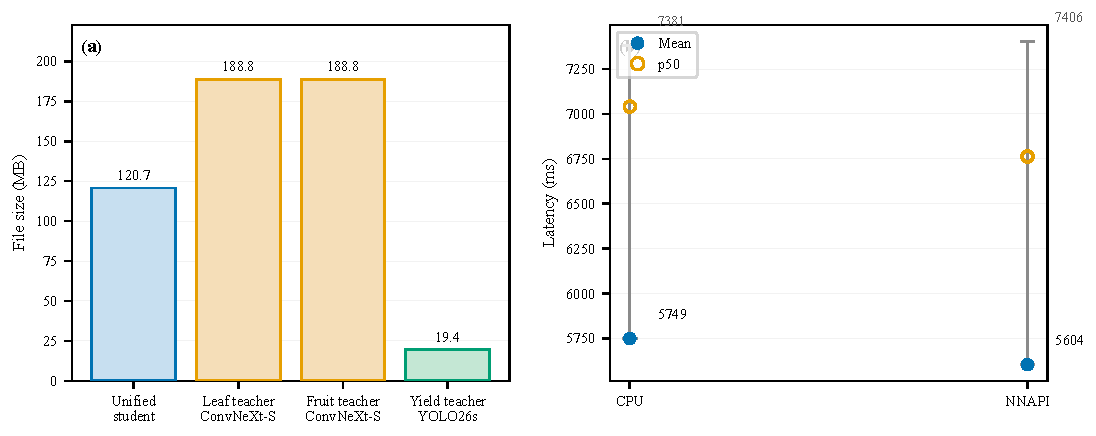
\includegraphics[width=\textwidth]{fig16_edge}
\caption{On-device cost on Samsung A17 5G. File sizes for the unified student versus teachers and latency by provider mode with identical predictions indicating central processing unit fallback. Accuracy on 30 yield and 20 pest images; latency distributions on 100 measured inferences per mode. Single run.}
\label{fig:edge}
\end{figure}

\FloatBarrier
%% Scientific Reports order: Introduction / Results / Discussion (no subheadings) / Methods.
%% For review this draft keeps Related/Methods early for readability; final
%% revision will move Sections~\ref{sec:methodology}--\ref{sec:experimental} after Discussion
%% without changing any numbers.
\section{Discussion}
\label{sec:discussion}

This section interprets what Tables~\ref{tab:final_results}--\ref{tab:edge}
and Figs.~\ref{fig:final}--\ref{fig:edge} jointly imply, rather than
repeating them. The held-out test shows a working unified model
with ceiling leaf and pest performance and strong counting
correlation. Contrary to expectation, removing
distillation matches or improves every metric and freezing the
backbone matches the proposed system. Distillation therefore shows no
gain under saturated teachers and ceiling tasks with fixed strengths
and one seed per configuration, while adaptation remains within estimated noise.
By contrast, static weighting collapses
fruit accuracy and thus supports adaptive weighting as essential.
Learned precisions are optimization coefficients rather than measures
of importance. On device, the remaining contribution is offline efficiency
with identical predictions across providers and no acceleration on the test hardware.

Agri-CNX-Edge unifies leaf, pest, fruit, and counting/detection in one
offline-capable DINOv3-ConvNeXt model with test 100.00\% leaf, 99.56\% pest
and 95.69\% fruit and counting mean absolute error (MAE) 3.53 at $r{=}0.85$ and $R^2{=}0.57$.
Against frozen at 95.69\% and 3.43 and without knowledge distillation (KD) at 99.14\% and 3.08, the
measured contribution is the unified efficiency system at 120.7\,MB offline
with identical predictions across central processing unit (CPU) and Neural Networks API (NNAPI) providers plus the validation of adaptive weighting
with static weighting at 70.26\% -- alongside a documented negative
distillation result under saturated-teacher conditions. Class-wise,
correlation, qualitative, and on-device evidence are measured;
confirmatory work is multi-seed repeats, static-weight completion, and
quantized builds.

\FloatBarrier
\section{Limitations and Future Work}
\label{sec:limitations}

Boundary conditions are stated plainly. The static-weighting run is
incomplete and is cited only as collapse evidence until completed.
Healthy fruit has no validation or test regions of interest (ROIs), so its generalization is
untested. The proposed system was evaluated from the latest checkpoint
rather than the best-validation epoch because only it was present at
evaluation time. Counting shows systematic undercounting that calls
for threshold calibration rather than ranking analysis. Latency tails
are approximate, battery readings are coarse and the latency subset is
train-sourced, while accuracy rests on validation and held-out test.
Pest phone images come from the training pool and serve only as
agreement sanity. A pilot on an older low-end phone was excluded as
impractical, so ultra-low-end deployment requires quantization.

Future work can investigate:

\begin{itemize}[leftmargin=*,itemsep=2pt,parsep=2pt]

\item completing the static-weighting run and repeating configurations
over seeds,

\item threshold calibration for dense clusters,

\item post-training quantization for ultra-low-end deployment,

\item Healthy-fruit data collection,

\item larger-scale orchard evaluation, and

\item comparison with single-task specialist baselines.

\end{itemize}

\section*{Acknowledgements}
We thank the providers of the public PlantVillage, Kaggle and Mendeley apple datasets used under their respective licenses. GPU access was provided by the Department of Computer Science and Engineering, Symbiosis Institute of Technology.

\section*{Author contributions}
A.B., A.B.H., E.B. and A.N. collected and curated the data. A.B., A.B.H., E.B. and A.G. performed data analysis and model development. A.B. and E.B. wrote the first draft of the manuscript. A.G. reviewed and edited the manuscript. All authors reviewed the manuscript and approved the submitted version. A.G. is the corresponding author and manages communication. No large language model meets authorship criteria; human authors retain full accountability.

\section*{Data Availability}
The datasets generated during and/or analysed during the current study are available as follows. Derived split files, cleaning logs, box labels and checkpoint index: [REPOSITORY-NAME-TO-BE-INSERTED, e.g. Zenodo — DOI-TO-BE-MINTED-ON-ACCEPTANCE; REVIEWER PRIVATE LINK-TO-BE-INSERTED]. Figure source data are provided as Supplementary Information. Third-party images were used under their licenses and are not redistributed: PlantVillage apple leaf mirror [LINK-LICENSE-ACCESSED-DATE-TO-BE-INSERTED], Kaggle apple fruit disease collection [LINK-LICENSE-ACCESSED-DATE-TO-BE-INSERTED], Mendeley apple fruit dataset v6 doi:10.17632/9zgkwwv9j8.6, Kaggle apple leaf and fruit segmentation collection [LINK-LICENSE-ACCESSED-DATE-TO-BE-INSERTED], Kaggle apple quality collection [LINK-LICENSE-ACCESSED-DATE-TO-BE-INSERTED]. Restrictions for third-party data are stated by the providers; derived data are available from the corresponding author on reasonable request once the repository is public.

\section*{Code Availability}
Custom training, evaluation, ONNX export and phone-benchmark code: [GITHUB-PRIVATE-URL-TO-BE-INSERTED, TO BE ARCHIVED ON ZENODO WITH DOI ON ACCEPTANCE; REVIEWER ZIP PROVIDED AS SUPPLEMENTARY]. Environment: PyTorch [VERSION-TO-BE-INSERTED], timm [VERSION-TO-BE-INSERTED], Albumentations [VERSION-TO-BE-INSERTED], scikit-learn [VERSION-TO-BE-INSERTED], ONNX opset 17. Commit hash: [HASH-TO-BE-INSERTED]. Inference uses the single 512-pixel student; fruit grading runs client-side from ROI-Align crops. Language polishing with an AI tool, if used beyond copy-editing, will be documented here with human verification; no AI system replaces author judgement.

\section*{Competing interests}
A.B., A.B.H., E.B., A.N. and A.G. declare no competing interests.

\section*{Funding}
Article processing charge funding is provided by Symbiosis International (Deemed University), Pune, India [GRANT-NUMBER-IF-APPLICABLE-TO-BE-INSERTED]. The funder had no role in conceptualization, design, data collection, analysis, decision to publish or manuscript preparation.

\section*{Ethics declarations: research involving plants}
No new plant or seed specimens were collected and no field trials were conducted. All leaf, pest, fruit and yield images come from the public third-party sources listed in Data Availability, used under their licenses. No wild-plant voucher specimen was required. Apple fruit boxes were produced semi-automatically with the base Segment Anything Model inside X-AnyLabeling [VERSIONS-TO-BE-INSERTED] followed by manual verification of every image before training or evaluation. This study includes no human participants, human data, identifiable images, vertebrate animals or clinical trials.

%% The Appendices part is started with the command \appendix;
%% appendix sections are then done as normal sections
% \appendix
% \FloatBarrier
% \section{Example Appendix Section}
% \label{app1}

%% If you have bib database file and want bibtex to generate the
%% bibitems, please use
%%
%%  \bibliographystyle{elsarticle-num}
%%  \bibliography{<your bibdatabase>}

%% else use the following coding to input the bibitems directly in the
%% TeX file.

%% Refer following link for more details about bibliography and citations.
%% https://en.wikibooks.org/wiki/LaTeX/Bibliography_Management

\FloatBarrier
%% SCI REP REFS: convert to Nature style on revision ([1] sequential, one work per number,
%% all authors if <=5 else first + et al., Roman article titles sentence-case, italic journal,
%% bold volume, full pages/article-number + DOI; move Kaggle/Mendeley/GitHub dataset URLs
%% from refs to Data Availability with licenses/access dates; verify each citation supports its statement).
\begin{thebibliography}{58}

%% References are listed in order of first citation for numbered style.

\bibitem{khan2022}
  S.~I. Khan, S.~M. Quadri, S.~Banday, and J.~L. Shah,
  ``Deep diagnosis: A real-time apple leaf disease detection system
  based on deep learning,''
  \textit{Computers and Electronics in Agriculture},
  vol.~198, 2022, Art.~no.~107093, doi:10.1016/j.compag.2022.107093. 

\bibitem{gao2022}
  F.~Gao et~al.,
  ``A novel apple fruit detection and counting methodology based on
  deep learning and trunk tracking in modern orchard,''
  \textit{Computers and Electronics in Agriculture},
  vol.~197, 2022, Art.~no.~107000, doi:10.1016/j.compag.2022.107000.

\bibitem{luan2025}
  P.~Luan et~al.,
  ``Accurate and efficient recognition of mixed diseases in apple leaves
  using a multi-task learning approach,''
  \textit{Agriculture}, vol.~16, no.~1, 2025, Art.~no.~71,
  doi:10.3390/agriculture16010071.

\bibitem{kang2024}
  R.~Kang et~al.,
  ``Toward real scenery: A lightweight tomato growth inspection
  algorithm for leaf disease detection and fruit counting,''
  \textit{Plant Phenomics}, vol.~6, 2024, Art.~no.~0174,
  doi:10.34133/plantphenomics.0174.

\bibitem{pmjdm2025}
  Y.~Li et~al.,
  ``PMJDM: a multi-task joint detection model for plant disease
  identification,''
  \textit{Frontiers in Plant Science}, vol.~16, 2025, Art.~no.~1599671,
  doi:10.3389/fpls.2025.1599671.

\bibitem{plantsds2026}
  S.~Sharma et~al.,
  ``A multi-feature fusion deep neural network with attention for
  multi-task crop monitoring,''
  \textit{Eng. Res. Express}, 2026, in press, doi:10.1088/2631-8695/ae5913.

\bibitem{cmtl2025}
  S.~Umirzakova et~al.,
  ``A unified transformer model for simultaneous cotton boll detection,
  pest damage segmentation, and phenological stage classification,''
  \textit{Drones}, vol.~9, no.~8, 2025, Art.~no.~555,
  doi:10.3390/drones9080555.

\bibitem{sood2025}
  V.~Sood et~al.,
  ``Towards automated crop protection: fusion of DenseNet121-ResNet50
  model for disease detection and pest recognition,''
  \textit{Int. J. Syst. Assur. Eng. Manag.}, 2025,
  doi:10.1007/s13198-025-02975-2.

\bibitem{damnet2024}
  H.~Zhang et~al.,
  ``Enhanced pest recognition using multi-task deep learning with the
  discriminative attention multi-network,''
  \textit{Applied Sciences}, vol.~14, no.~13, 2024, Art.~no.~5543,
  doi:10.3390/app14135543.

\bibitem{wen2022}
  C.~Wen et~al.,
  ``Pest-YOLO: A model for large-scale multi-class dense and tiny pest
  detection and counting,''
  \textit{Frontiers in Plant Science}, vol.~13, 2022, Art.~no.~973985,
  doi:10.3389/fpls.2022.973985.

\bibitem{plante2024}
  O.~Appiah et~al.,
  ``PlanteSaine: An artificial intelligent empowered mobile application
  for pests and disease management,''
  \textit{Agriculture}, vol.~14, no.~8, 2024, Art.~no.~1252,
  doi:10.3390/agriculture14081252.

\bibitem{wang2023ulen}
  B.~Wang et~al.,
  ``An ultra-lightweight efficient network for image-based plant disease
  and pest infection detection,''
  \textit{Precision Agriculture}, vol.~24, 2023, pp.~1836--1861,
  doi:10.1007/s11119-023-10020-0.

\bibitem{schuler2022edge}
  J.~Schuler et~al.,
  ``Plant disease detection model for edge computing devices,''
  \textit{Frontiers in Plant Science}, vol.~14, 2023, Art.~no.~1308528,
  doi:10.3389/fpls.2023.1308528.

\bibitem{bai2024dinov2}
  C.~Bai et~al.,
  ``DINOV2-FCS: a model for fruit leaf disease classification and
  severity prediction,''
  \textit{Frontiers in Plant Science}, vol.~15, 2024, Art.~no.~1475282,
  doi:10.3389/fpls.2024.1475282.

\bibitem{huang2025econv}
  X.~Huang et~al.,
  ``EConv-ViT: A strongly generalized apple leaf disease classification
  model based on the fusion of ConvNeXt and Transformer,''
  \textit{Inf. Process. Agric.}, 2025, doi:10.1016/j.inpa.2025.03.001.

\bibitem{simeoni2025}
  O.~Sim{\'e}oni et~al.,
  ``DINOv3,''
  \textit{Trans. Mach. Learn. Res.}, 2026.

\bibitem{huang2023}
  Q.~Huang et~al.,
  ``Knowledge distillation facilitates the lightweight and efficient
  plant diseases detection model,''
  \textit{Plant Phenomics},
  vol.~5, 2023, Art.~no.~0062, doi:10.34133/plantphenomics.0062.

\bibitem{kendall2018}
  A.~Kendall, Y.~Gal, and R.~Cipolla,
  ``Multi-task learning using uncertainty to weigh losses for scene
  geometry and semantics,''
  in \textit{Proceedings of the IEEE/CVF Conference on Computer Vision
  and Pattern Recognition (CVPR)}, 2018, pp.~7482--7491,
  doi:10.1109/CVPR.2018.00781.

\bibitem{chen2018}
  Z.~Chen, V.~Badrinarayanan, C.-Y.~Lee, and A.~Rabinovich,
  ``GradNorm: Gradient normalization for adaptive loss balancing in
  deep multitask networks,''
  in \textit{Proceedings of the International Conference on Machine
  Learning (ICML)}, 2018, pp.~794--803.

\bibitem{liu2021cagrad}
  B.~Liu, X.~Liu, X.~Jin, P.~Stone, and Q.~Liu,
  ``Conflict-averse gradient descent for multi-task learning,''
  in \textit{Advances in Neural Information Processing Systems
  (NeurIPS)}, vol.~34, 2021.

\bibitem{reddi2022}
  V.~J.~Reddi et~al.,
  ``MLPerf mobile inference benchmark: An industry-standard open-source
  machine learning benchmark for on-device AI,''
  in \textit{Proceedings of Machine Learning and Systems (MLSys)},
  vol.~4, 2022, pp.~352--369.

\bibitem{liumd2022}
  X.~Liu et~al.,
  ``A comprehensive benchmark of deep learning libraries on mobile
  devices,''
  in \textit{Proceedings of the ACM Web Conference (WWW)}, 2022,
  doi:10.1145/3485447.3512148.



\bibitem{jin2025}
  T.~Jin, X.~Han, P.~Wang, Z.~Zhang, J.~Guo, and F.~Ding,
  ``Enhanced deep learning model for apple detection, localization, and
  counting in complex orchards for robotic arm-based harvesting,''
  \textit{Smart Agricultural Technology},
  vol.~10, 2025, Art.~no.~100784, doi:10.1016/j.atech.2025.100784.

\bibitem{hani2020}
  N.~Hani, P.~Roy, and V.~Isler,
  ``A comparative study of fruit detection and counting methods for yield
  mapping in apple orchards,''
  \textit{J. Field Robot.}, vol.~37, no.~2, 2020, pp.~263--282,
  doi:10.1002/rob.21902.

\bibitem{mohanty2016}
  S.~P. Mohanty, D.~P. Hughes, and M.~Salath{\'e},
  ``Using deep learning for image-based plant disease detection,''
  \textit{Frontiers in Plant Science},
  vol.~7, 2016, Art.~no.~1419, doi:10.3389/fpls.2016.01419.

\bibitem{ferentinos2018}
  K.~P. Ferentinos,
  ``Deep learning models for plant disease detection and diagnosis,''
  \textit{Computers and Electronics in Agriculture},
  vol.~145, 2018, pp.~311--318, doi:10.1016/j.compag.2018.01.009.

\bibitem{dhaka2021}
  V.~S. Dhaka et~al.,
  ``A survey of deep convolutional neural networks applied for
  prediction of plant leaf diseases,''
  \textit{Sensors}, vol.~21, no.~14, 2021, Art.~no.~4749,
  doi:10.3390/s21144749.

\bibitem{liu2021}
  J.~Liu and X.~Wang,
  ``Plant diseases and pests detection based on deep learning:
  a review,''
  \textit{Plant Methods},
  vol.~17, 2021, Art.~no.~22, doi:10.1186/s13007-021-00722-9.

\bibitem{shoaib2025}
  Shoaib et~al.,
  ``Leveraging deep learning for plant disease and pest detection:
  a comprehensive review and future directions,''
  \textit{Frontiers in Plant Science},
  vol.~16, 2025, Art.~no.~1538163, doi:10.3389/fpls.2025.1538163.

\bibitem{banerjee2025}
  S.~Banerjee, T.~Mallick, A.~Chakroborty, H.~N. Saha, and N.~T. Takur,
  ``Evaluation of state-of-the-art deep learning techniques for plant
  disease and pest detection,''
  \textit{Comput. Mater. Contin.}, vol.~85, 2025, pp.~121--180,
  doi:10.32604/cmc.2025.065250.

\bibitem{wu2019ip102}
  X.~Wu et~al.,
  ``IP102: A large-scale benchmark dataset for insect pest recognition,''
  in \textit{Proc. IEEE/CVF Conf. Comput. Vis. Pattern Recognit. (CVPR)},
  2019, doi:10.1109/CVPR.2019.00899.

\bibitem{picon2018}
  A.~Picon, A.~Alvarez-Gila, M.~Seitz, A.~Ortiz-Barredo, J.~Echazarra,
  and A.~Johannes,
  ``Deep convolutional neural networks for mobile capture
  device-based crop disease classification in the wild,''
  \textit{Computers and Electronics in Agriculture},
  vol.~161, 2019, pp.~280--290, doi:10.1016/j.compag.2018.04.002.

\bibitem{janarthan2022}
  S.~Janarthan et~al.,
  ``P2OP--Plant Pathology on Palms: A deep learning-based mobile
  solution for in-field plant disease detection,''
  \textit{Computers and Electronics in Agriculture},
  vol.~202, 2022, Art.~no.~107371, doi:10.1016/j.compag.2022.107371.

\bibitem{picon2019}
  A.~Picon et~al.,
  ``Crop conditional convolutional neural networks for massive
  multi-crop plant disease classification over cell phone acquired
  images taken on real field conditions,''
  \textit{Computers and Electronics in Agriculture},
  vol.~167, 2019, Art.~no.~105093, doi:10.1016/j.compag.2019.105093.

\bibitem{he2016}
  K.~He, X.~Zhang, S.~Ren, and J.~Sun,
  ``Deep residual learning for image recognition,''
  in \textit{Proceedings of the IEEE Conference on Computer Vision
  and Pattern Recognition (CVPR)}, 2016, pp.~770--778,
  doi:10.1109/CVPR.2016.90.

\bibitem{liu2022}
  Z.~Liu et~al.,
  ``A ConvNet for the 2020s,''
  in \textit{Proceedings of the IEEE/CVF Conference on Computer Vision
  and Pattern Recognition (CVPR)}, 2022, pp.~11976--11986,
  doi:10.1109/CVPR52688.2022.01167.

\bibitem{swin2021}
  Z.~Liu et~al.,
  ``Swin Transformer: Hierarchical vision transformer using shifted
  windows,''
  in \textit{Proceedings of the IEEE/CVF International Conference on
  Computer Vision (ICCV)}, 2021, pp.~10012--10022,
  doi:10.1109/ICCV48922.2021.00986.

\bibitem{dosovitskiy2020}
  A.~Dosovitskiy et~al.,
  ``An image is worth 16x16 words: Transformers for image recognition
  at scale,''
  in \textit{Proceedings of the International Conference on Learning
  Representations (ICLR)}, 2021.

\bibitem{caron2021}
  M.~Caron et~al.,
  ``Emerging properties in self-supervised vision transformers,''
  in \textit{Proceedings of the IEEE/CVF International Conference on
  Computer Vision (ICCV)}, 2021, pp.~9650--9660,
  doi:10.1109/ICCV48922.2021.00951.

\bibitem{oquab2023}
  M.~Oquab et~al.,
  ``DINOv2: Learning robust visual features without supervision,''
  \textit{Trans. Mach. Learn. Res.}, 2024.

\bibitem{tan2019}
  M.~Tan and Q.~V.~Le,
  ``EfficientNet: Rethinking model scaling for convolutional neural
  networks,''
  in \textit{Proceedings of the International Conference on Machine
  Learning (ICML)}, 2019, pp.~6105--6114.

\bibitem{howard2019}
  A.~Howard et~al.,
  ``Searching for MobileNetV3,''
  in \textit{Proceedings of the IEEE/CVF International Conference on
  Computer Vision (ICCV)}, 2019, pp.~1314--1324,
  doi:10.1109/ICCV.2019.00140.

\bibitem{redmon2016}
  J.~Redmon, S.~Divvala, R.~Girshick, and A.~Farhadi,
  ``You only look once: Unified, real-time object detection,''
  in \textit{Proceedings of the IEEE Conference on Computer Vision
  and Pattern Recognition (CVPR)}, 2016, pp.~779--788,
  doi:10.1109/CVPR.2016.91.

\bibitem{jocher2020}
  G.~Jocher et~al.,
  ``Ultralytics YOLOv5,''
  software release, 2020.

\bibitem{lin2017}
  T.-Y.~Lin, P.~Doll{\'a}r, R.~Girshick, K.~He, B.~Hariharan, and
  S.~Belongie,
  ``Feature pyramid networks for object detection,''
  in \textit{Proceedings of the IEEE Conference on Computer Vision
  and Pattern Recognition (CVPR)}, 2017, pp.~2117--2125,
  doi:10.1109/CVPR.2017.106.

\bibitem{hu2021}
  E.~J.~Hu et~al.,
  ``LoRA: Low-rank adaptation of large language models,''
  in \textit{Proceedings of the International Conference on Learning
  Representations (ICLR)}, 2022.

\bibitem{han2016}
  S.~Han, H.~Mao, and W.~J. Dally,
  ``Deep compression: Compressing deep neural networks with pruning,
  trained quantization and Huffman coding,''
  in \textit{Proc. Int. Conf. Learn. Represent. (ICLR)}, 2016.

\bibitem{jacob2018}
  B.~Jacob et~al.,
  ``Quantization and training of neural networks for efficient
  integer-arithmetic-only inference,''
  in \textit{Proc. IEEE Conf. Comput. Vis. Pattern Recognit. (CVPR)},
  2018, doi:10.1109/CVPR.2018.00286.

\bibitem{vandenhende2022}
  S.~Vandenhende, S.~Georgoulis, W.~Van~Gansbeke, M.~Proesmans,
  D.~Dai, and L.~Van~Gool,
  ``Multi-task learning for dense prediction tasks: A survey,''
  \textit{IEEE Transactions on Pattern Analysis and Machine
  Intelligence}, vol.~44, no.~7, 2022, pp.~3614--3633,
  doi:10.1109/TPAMI.2021.3054719.

\bibitem{sener2018}
  O.~Sener and V.~Koltun,
  ``Multi-task learning as multi-objective optimization,''
  in \textit{Adv. Neural Inf. Process. Syst.}, vol.~31, 2018.

\bibitem{yu2020}
  T.~Yu et~al.,
  ``Gradient surgery for multi-task learning,''
  in \textit{Adv. Neural Inf. Process. Syst.}, vol.~33, 2020.


\bibitem{leafkaggle}
  ``PlantVillage dataset (mirror),''
  Kaggle. \url{https://www.kaggle.com/datasets/abdallahalidev/plantvillage-dataset}.

\bibitem{fruitkaggle}
  ``Apple fruit disease images dataset,''
  Kaggle. \url{https://www.kaggle.com/datasets/anilsandhii/apple-fruit-disease-images-dataset}.

\bibitem{fruitmendeley}
  ``Apple fruit dataset,''
  Mendeley Data, v6. \url{https://data.mendeley.com/datasets/9zgkwwv9j8/6},
  doi:10.17632/9zgkwwv9j8.6.

\bibitem{pestkaggle}
  ``Apple leaf and fruit disease segmentation dataset,''
  Kaggle. \url{https://www.kaggle.com/datasets/yaldanz/apple-leaf-and-fruit-disease-segmenattion}.

\bibitem{applequality}
  ``Apple quality dataset,''
  Kaggle. \url{https://www.kaggle.com/datasets/snehamahata/apple-quality-dataset}.

\bibitem{sam2023}
  A.~Kirillov et~al.,
  ``Segment Anything,''
  in \textit{Proc. IEEE/CVF Int. Conf. Comput. Vis. (ICCV)}, 2023,
  doi:10.1109/ICCV51070.2023.00371.

\bibitem{xanylabeling2023}
  W.~Wang,
  ``Advanced auto labeling solution with added features,''
  GitHub repository, CVHub, 2023.
  \url{https://github.com/CVHub520/X-AnyLabeling}.

\end{thebibliography}
\end{document}

\endinput
%%
%% End of file `main.tex'.
